% =============================================================================
%  몬테카를로법 — 『밑바닥부터 시작하는 딥러닝 4』 5장 정리
%
%  컴파일:  tectonic -X compile ch05_mc.tex
%  (XeLaTeX 계열 엔진 + kotex + NanumGothic 필요)
%  그림:    python ch05/paper/fig_mc.py  로 그림 두 개 생성
% =============================================================================
\documentclass[11pt,a4paper]{article}

\usepackage{kotex}
\usepackage{amsmath,amssymb}
\usepackage{amsthm}
\usepackage{graphicx}
\usepackage{booktabs}
\usepackage{multirow}
\usepackage{listings}
\usepackage{xcolor}
\usepackage{algorithm}
\usepackage{algpseudocode}
\usepackage[margin=27mm,top=28mm,bottom=28mm]{geometry}
\usepackage[labelsep=period,font=small,labelfont=bf]{caption}
\usepackage{enumitem}
\usepackage[hidelinks]{hyperref}

% ---- 한글 글꼴 -------------------------------------------------------------
\setmainhangulfont{NanumGothic}
\setsanshangulfont{NanumGothic}
\setmonohangulfont[Scale=MatchLowercase]{NanumGothic}

% ---- 한글 캡션 이름 ---------------------------------------------------------
\renewcommand{\figurename}{그림}
\renewcommand{\tablename}{표}
\renewcommand{\refname}{참고문헌}
\renewcommand{\abstractname}{초록}
\renewcommand{\contentsname}{차례}
\floatname{algorithm}{알고리즘}
\renewcommand{\algorithmicrequire}{\textbf{입력:}}
\renewcommand{\algorithmicensure}{\textbf{출력:}}

% ---- 정리 환경 -------------------------------------------------------------

% ---- 코드 리스팅 -----------------------------------------------------------
\definecolor{codekw}{RGB}{0,86,153}
\definecolor{codecm}{RGB}{112,128,144}
\definecolor{codestr}{RGB}{163,21,21}
\definecolor{codebg}{RGB}{249,249,250}
% 주의: listings는 라틴 문자를 단어 단위로 버퍼링했다가 출력하는데, kotex 환경에서
% 한글이 섞이면 버퍼가 한글 뒤에 flush되어 글자 순서가 뒤바뀐다("q에" -> "에q").
% 그래서 한글 주석은 escapeinside 구간에서 일반 조판 모드로 넘겨 처리한다.
\lstdefinestyle{py}{
  language=Python,
  escapeinside={<@}{@>},
  basicstyle=\ttfamily\small,
  keywordstyle=\color{codekw}\bfseries,
  commentstyle=\color{codecm}\itshape,
  stringstyle=\color{codestr},
  backgroundcolor=\color{codebg},
  frame=single,
  rulecolor=\color{black!25},
  framesep=5pt,
  columns=fullflexible,
  keepspaces=true,
  showstringspaces=false,
  breaklines=true,
  captionpos=b,
  numbers=none,
  aboveskip=1.1em,
  belowskip=0.6em,
}
\lstset{style=py}
\renewcommand{\lstlistingname}{코드}

% ---- 플로트 배치 -----------------------------------------------------------
% 기본값(topfraction 0.7, floatpagefraction 0.5)으로는 표·그림이 본문과 같은 쪽에
% 못 앉고 한데 몰려 '플로트 전용 쪽'을 만든다. 한 쪽이 플로트로 채워질 수 있는 몫을
% 늘리고, 플로트 전용 쪽의 최소 충전율을 올려 성긴 플로트 쪽이 생기지 않게 한다.
\renewcommand{\topfraction}{0.88}
\renewcommand{\bottomfraction}{0.70}
\renewcommand{\textfraction}{0.12}
\renewcommand{\floatpagefraction}{0.80}
\setcounter{topnumber}{3}
\setcounter{bottomnumber}{2}
\setcounter{totalnumber}{5}

% ---- 그림 경로 -------------------------------------------------------------
\graphicspath{{../../images/figures/}{../../images/equations/}{./}}

% ---- 편의 매크로 -----------------------------------------------------------
\newcommand{\E}{\mathbb{E}}
\newcommand{\Sset}{\mathcal{S}}
\newcommand{\Aset}{\mathcal{A}}
\newcommand{\bookfig}[1]{\textit{출처: 원서 그림 #1.}}
\newcommand{\cmt}[1]{\textcolor{codecm}{#1}}   % 리스팅 안의 한글 주석

% ---- 차례의 절 번호 폭 -------------------------------------------------------
% \thesection 이 "5.1" 처럼 두 토막이라 article 기본 폭(1.5em)으로는 번호와 제목이
% 붙어 버린다. 번호 상자를 넓혀 준다.
\makeatletter
\renewcommand*\l@section[2]{%
  \ifnum \c@tocdepth >\z@
    \addpenalty\@secpenalty
    \addvspace{1.0em \@plus\p@}%
    \setlength\@tempdima{2.8em}%
    \begingroup
      \parindent \z@ \rightskip \@pnumwidth
      \parfillskip -\@pnumwidth
      \leavevmode \bfseries
      \advance\leftskip\@tempdima \hskip -\leftskip
      #1\nobreak\hfil \nobreak\hb@xt@\@pnumwidth{\hss #2}\par
    \endgroup
  \fi}
\renewcommand*\l@subsection{\@dottedtocline{2}{2.8em}{3.4em}}
\makeatother

% ---- 절 번호를 원서 5장 목차에 맞춤 -----------------------------------------
% 번호 있는 절은 원서/README의 5.1~5.6과 정확히 대응한다. 서론과 재현 정보는
% 번호를 붙이지 않고, 하위 절보다 깊은 제목은 번호와 차례에서 뺀다.
\renewcommand{\thesection}{5.\arabic{section}}
\setcounter{secnumdepth}{2}
\setcounter{tocdepth}{2}


\title{\bfseries 몬테카를로법\\[2mm]
\large 기댓값을 표본 평균으로 바꾸기: 모델 없는 평가와 제어,
그리고 ``누구의 경험으로 배우는가''라는 하나의 축}
\author{sajacaros\\\small \texttt{sajacall82@naver.com}}
\date{2026년 9월 7일}

\begin{document}
\maketitle

\begin{abstract}
\noindent
앞 장의 동적 프로그래밍(DP)은 벨만 방정식의 등호를 갱신식으로 바꿔 읽어 가치 함수를 얻었지만, 그
갱신식 안에는 환경 모델 $p$와 $r$가 그대로 들어 있었다. 코드가 \lstinline|env.next_state()|와
\lstinline|env.reward()|를 직접 부른다는 사실이 그 전제의 표현이다. 현실의 문제는 그 표를 내주지
않는다. \emph{몬테카를로법}(MC법)은 전제를 바꾸는 대신 계산을 바꾼다. 가치 함수는 수익의
기댓값이므로, 분포를 알아야만 구할 수 있는 것이 아니라 \emph{여러 번 해보고 평균을 내면} 된다.
본고는 이 한 줄의 교체에서 출발하여 \emph{MC 정책 평가}, \emph{$\varepsilon$-탐욕과 고정값 $\alpha$를
붙인 온-정책 MC 제어}, \emph{중요도 샘플링을 쓰는 오프-정책 MC 제어}를 정리하고, 세 알고리즘이
``누구의 경험으로 배우는가''라는 하나의 축 위의 서로 다른 지점임을 보인다.
원서\cite{dlfs4} 5장은 예제 코드를 제공하므로 본고는 그것을 그대로 쓰되, 원서가 관찰로만 남기거나
아예 짚지 않은 자리에 다섯 가지 논의를 더하였다. 절 구성은 원서 5장의 목차를 그대로 따르며, 더한
논의는 그것이 필요해지는 자리의 본문에 ``[보충]''으로 결론만 적고 표와 유도는 부록에 모았다.
앞의 둘은 이름과 방식을 밝히는 것으로, ``몬테카를로''라는 말의 유래와 강화 학습이 그것을 쓰는 좁은
뜻을 적고, 예제 코드가 말없이 택한 \emph{모든 방문} 방식이 교과서의 \emph{첫 방문} 방식과 어떻게
다른지를 짚는다. 나머지 셋은 실측으로 답한다. 표본 오차는 $1/\sqrt{n}$로만 줄어들어, 앞 장의 DP가
백업 $1{,}104$회로 얻은 정확도에 MC법이 이르려면 약 $3.9\times10^{6}$걸음이 필요하다. 고정값
$\alpha$는 잔차의 표준편차를 $\sqrt{\alpha/(2-\alpha)}\,\sigma_G$라는 바닥에 멈춰 세우지만, 제어에서는
그럼에도 $1/n$ 평균보다 낫다. 오프-정책 예제의 대상 정책은 \emph{결정적}이어서 갱신의 절반
이상($53.1$--$65.5\%$)에서 중요도 가중치 $\rho$가 이미 $0$이며, 이것이 오프-정책이 ``정책은 더 잘
맞히면서 값은 더 부정확한'' 까닭이다.

\vspace{2mm}
\noindent\textbf{주제어:} 강화 학습, 몬테카를로법, 샘플 모델, 첫 방문/모든 방문, $\varepsilon$-탐욕
정책, 지수 이동 평균, 온-정책, 오프-정책, 중요도 샘플링
\end{abstract}

\tableofcontents
\vspace{4mm}

% =============================================================================
\section*{서론}
\addcontentsline{toc}{section}{서론}
% =============================================================================

\subsection*{모델을 아는 것에서 해보는 것으로}

앞 장\cite{ch04}에서 벨만 방정식의 등호를 대입으로 바꿔 읽어 반복적 정책 평가, 정책 반복법, 가치
반복법을 얻었다. 세 알고리즘의 갱신식은 모두
\begin{equation*}
  V_{k+1}(s) = \sum_{a} \pi(a\mid s) \sum_{s'} p(s'\mid s,a)
               \bigl\{\, r(s,a,s') + \gamma\, V_k(s') \,\bigr\}
\end{equation*}
의 모양이었고, 여기에는 $p$와 $r$가 그대로 들어 있다. 이 합을 계산하려면 ``어느 상태로 얼마의 확률로
가는지''와 ``그때 얼마를 받는지''를 미리 알아야 한다. 앞 장의 예제가 \lstinline|env.next_state()|와
\lstinline|env.reward()|를 부르는 자리가 정확히 그 지점이다.

현실의 문제는 그 표를 내주지 않는다. 바둑의 규칙은 알아도 모든 국면의 전이를 표로 적을 수 없고,
로봇이 바닥과 어떻게 마찰하는지는 애초에 식으로 주어지지 않는다. 그래서 이 장은 전제를 바꾼다.
가진 것은 ``행동을 넣으면 다음 상태와 보상을 돌려주는'' 장치 하나뿐이라고 두는 것이다.

이 장이 바꾸는 것은 위 갱신식의 $\sum_{s'} p(s'\mid s,a)$ 하나다. 상태 가치 함수의 정의가 애초에
기댓값이라는 데서 출발한다.
\begin{equation*}
  v_\pi(s) = \E_\pi\bigl[\, G_t \mid S_t = s \,\bigr],
  \qquad G_t = R_t + \gamma R_{t+1} + \gamma^2 R_{t+2} + \cdots
\end{equation*}
기댓값을 구하는 길은 둘이다. 분포를 알고 $\sum_x x\,p(x)$를 계산하거나, 표본을 여럿 뽑아 산술 평균을
내거나. 앞 장이 앞의 길이고 이 장이 뒤의 길이다. 뒤의 길을 \emph{몬테카를로법}이라 하며, 그것이
참값에 다가간다는 근거는 큰 수의 법칙이다.

교체의 대가는 셋이다. 첫째, 답이 근사치이고 실행할 때마다 달라진다. 오차는 문턱으로 정하는 것이
아니라 표본 수로 정해지며 $1/\sqrt{n}$로만 줄어든다. 둘째, 수익 $G_t$를 알려면 에피소드가 끝나야
하므로 \emph{일회성 과제}에만 쓸 수 있다. 셋째, 모든 상태를 빠짐없이 훑는 DP와 달리 \emph{가본 곳만}
배운다. 이 셋이 각각 구현과 제어와 오프-정책에서 문제가 되는 자리를 만든다.

\subsection*{본고의 구성과 기여}

본고는 원서 5장의 목차를 그대로 따른다. 주사위 예제로 몬테카를로법의 뼈대와 증분 평균을 세우고,
그것을 정책 평가에 옮기며 한 에피소드에서 모든 상태의 수익을 뽑아내는 뒤에서부터 계산하기를 얻는다.
이어 $3\times4$ 그리드 월드에 구현하고, 평가에 개선을 붙여 제어로 넘어가며 $\varepsilon$-탐욕 정책과
고정값 $\alpha$ 두 처방을 붙인다. 마지막으로 행동하는 정책과 평가할 정책을 갈라 중요도 샘플링으로
잇는다.

원서 5장은 예제 코드를 제공하므로 본고는 그것을 그대로 쓰되, 원서가 관찰로만 남기거나 아예 짚지 않은
다섯 자리에 논의를 더하였다. 더한 논의는 그것이 필요해지는 자리의 본문에 ``[보충]''으로 표시하고
결론만 몇 줄로 적었으며, 그것을 떠받치는 표와 유도는 부록에 모았다. 줄거리를 따라가는 독자는 [보충]만
읽고 지나가면 되고, 근거가 궁금한 자리에서만 부록을 펼치면 된다.

큰 수의 법칙과 중심 극한 정리의 증명, 첫 방문 추정량의 불편성 증명, 지수 이동 평균의 점근 분산
유도 같은 대목은 이 장의 줄거리를 따라가는 데 꼭 필요하지 않아 덜어내고 결과와 그 뜻만 남겼다.
% =============================================================================
\section{몬테카를로법 기초}
\label{sec:basic}
% =============================================================================

\subsection{주사위 눈의 합}
\label{sec:dice}

주사위 두 개를 던져 나온 눈의 합의 기댓값을 구한다. 답은 $7$이고 구하는 길은 둘이다.

\begin{figure}[htbp]
\centering
\begin{minipage}[t]{0.52\linewidth}\centering
  \includegraphics[width=\linewidth]{{fig 5-1}.png}
\end{minipage}\hfill
\begin{minipage}[t]{0.44\linewidth}\centering
  \includegraphics[width=\linewidth]{{fig 5-2}.png}
\end{minipage}
\caption{두 번 던지는 과정을 전개한 나무(왼쪽)와 그 $36$가지를 합계별로 센 확률분포(오른쪽).
왼쪽 나무의 잎이 $36$개이고 주사위가 $n$개면 $6^n$개다. 오른쪽에서 $7$이 $6/36$으로 가장 많으며
$\sum_x x\,p(x)=7$이다. \bookfig{5-1, 5-2}}
\label{fig:dice}
\end{figure}

앞의 길, 곧 그림~\ref{fig:dice} 오른쪽의 표를 만들어 $\sum_x x\,p(x)$를 계산하는 것이 4장까지의
방식이다. 이 길이 막히는 자리는 둘이다. 하나는 경우의 수가 폭발할 때다. 주사위가 셋이면 잎이
$216$개, 열이면 $6^{10}\approx6.05\times10^7$개다. 다른 하나는 애초에 분포를 모를 때다. 눈이 고르지
않게 깎인 주사위라면 그림~\ref{fig:dice} 오른쪽을 그릴 방법이 없다.

뒤의 길은 그냥 던지는 것이다. 여러 번 던져 나온 합을 산술 평균한다. 표를 만들 필요도, 분포를 알
필요도 없다. 필요한 것은 던질 수 있다는 것뿐이다.

\subsection{분포 모델과 샘플 모델}
\label{sec:models}

두 길의 차이는 환경을 어떤 형태로 갖고 있느냐의 차이다.

\begin{figure}[htbp]
\centering
\includegraphics[width=0.56\linewidth]{{fig 5-3}.png}
\caption{왼쪽은 표를 내놓고 오른쪽은 굴린 결과 하나를 내놓는다. 왼쪽이 분포 모델, 오른쪽이 샘플
모델이다. \bookfig{5-3}}
\label{fig:models}
\end{figure}

\begin{table}[htbp]
\centering
\caption{분포 모델과 샘플 모델. 샘플 모델이 훨씬 만들기 쉽다는 것이 이 장의 출발점이다.}
\label{tab:models}
\small
\begin{tabular}{@{}lll@{}}
\toprule
 & 분포 모델(distribution model) & 샘플 모델(sample model) \\
\midrule
가진 것   & 확률분포 전체                      & 표본을 만들어 내는 능력만 \\
예        & $p(s'\mid s,a)$와 $r$의 표         & 게임 시뮬레이터, 물리 엔진, 실제 로봇 \\
쓰는 방법 & 4장 동적 프로그래밍                & 5장 몬테카를로법 \\
코드      & \lstinline|env.next_state(s, a)|   & \lstinline|env.step(a)| \\
\bottomrule
\end{tabular}
\end{table}

주사위를 굴리는 함수는 세 줄이면 되지만 두 눈의 합의 분포표를 만들려면 $36$가지를 다 세어야 한다.
분포 모델이 있으면 샘플 모델은 언제나 만들 수 있지만 반대는 성립하지 않는다. 샘플 모델이 더 약한
가정이고, 그래서 더 널리 쓰인다.

\subsection{몬테카를로법 구현}
\label{sec:dice-impl}

표본 평균을 구하는 방법도 두 가지다. 매번 전부 더해 나누는 방식과 \emph{증분} 방식이다.

\begin{figure}[htbp]
\centering
\includegraphics[width=0.6\linewidth]{{fig 5-4}.png}
\caption{1.3.2절에서 본 두 가지 평균 계산법. 아래쪽 식
$V_n = V_{n-1} + \frac{1}{n}(s_n - V_{n-1})$에는 $s_1,\dots,s_{n-1}$이 등장하지 않는다. 표본을
저장할 필요가 없다는 뜻이다. \bookfig{5-4}}
\label{fig:incremental}
\end{figure}

\begin{lstlisting}[caption={증분 방식의 표본 평균 (\texttt{s01\_dice.py})},label={lst:dice}]
def sample(dices=2):
    x = 0
    for _ in range(dices):
        x += np.random.choice([1, 2, 3, 4, 5, 6])
    return x

trial = 1000
V, n = 0, 0
for _ in range(trial):
    s = sample()
    n += 1
    V += (s - V) / n     <@\cmt{\# 증분 방식: 과거 표본을 들고 있지 않다}@>
\end{lstlisting}

$1{,}000$번 시행하면 $6.92$ 근처가 나온다. 참값 $7$에 가깝지만 정확히 $7$은 아니고, 실행할 때마다
다르다. 이 어긋남의 크기는 미리 계산할 수 있다. 주사위 하나의 분산이 $35/12$이므로 두 개의 합은
$\sigma^2 = 35/6$, $\sigma = 2.4152$다. 표본 평균의 표준오차는
\begin{equation*}
  \mathrm{SE}(n) = \frac{\sigma}{\sqrt{n}}
\end{equation*}
이므로 $n=1000$에서 $0.0764$다. 관측된 어긋남 $0.084$는 그 $1.1$배로, 표본 평균이 통상적으로 흔들리는
폭 안에 있다. $\sigma/\sqrt{n}$이라는 이 모양에서 이 장 전체를 관통하는 사실 하나가 따라 나온다. \emph{오차를 열 배
줄이려면 시행을 백 배 늘려야 한다.} 이 느림이 뒤에서 다시 문제가 된다.

\subsubsection{[보충] 왜 ``몬테카를로''인가}
\label{sec:whymc}

앞 장에서 ``동적 프로그래밍''이라는 이름이 기법의 성질과 별 관계가 없다는 것을 보았다. 이 이름도
사정이 비슷하다.

\paragraph{이름의 유래.}
1946년 로스앨러모스의 스타니스와프 울람이 병을 앓고 회복하는 동안 카드놀이 솔리테어를 하다가
``이 판이 풀릴 확률은 얼마인가''를 물었다. 모든 배열을 세어 계산하는 길은 원리상 열려 있으나 경우의
수가 감당할 수 없이 크다는 것을 알고, 여러 판을 실제로 늘어놓아 세어 보는 편이 낫겠다고 생각한
것이 시작이다\cite{ulam}. 울람은 이 착상을 폰 노이만에게 말했고 둘은 이를 중성자 확산 계산에 적용할
계획을 세웠다. 연구가 기밀이라 암호명이 필요했는데, 동료 니컬러스 메트로폴리스가 \emph{Monte Carlo}를
제안하였다. 울람의 삼촌이 도박을 하러 모나코의 몬테카를로 카지노에 가겠다며 친척들에게 돈을 빌리곤
했다는 사연에서 따온 이름이다. 기법을 처음 공개한 논문이 메트로폴리스와 울람의 1949년
글\cite{metropolis}이다. 요컨대 이 이름도 기법의 성질을 담으려고 지은 것이 아니며, 이름에서 내용을
읽어내려 애쓸 일이 아니다. 다만 앞 장의 ``동적 프로그래밍''이 예산을 얻기 위한 위장이었던 것과 달리
이쪽은 우연이 만든 별명에 가깝다.

\paragraph{기법으로서의 넓은 뜻.}
내용 쪽의 정의는 넓다. \emph{난수를 써서 수치적인 답을 얻는 방법}은 모두 몬테카를로법이다. 원주율을
사각형 안에 점을 뿌려 재는 것도, 고차원 적분을 무작위 점의 평균으로 구하는 것도, 통계물리의
메트로폴리스 알고리즘도 여기 든다. 대비되는 이름이 \emph{라스베이거스 알고리즘}이다. 라스베이거스
쪽은 답이 언제나 옳고 걸리는 시간이 무작위인 반면, 몬테카를로 쪽은 걸리는 시간이 정해져 있고 답이
무작위다. 이 장의 방법이 뒤쪽인 것은 앞 절에서 본 그대로다. 시행 횟수를 정해 놓고 돌리면 반드시
그만큼에 끝나지만, 나오는 값은 실행할 때마다 다르다.

\paragraph{강화 학습에서의 좁은 뜻.}
서튼과 바르토\cite{sutton}는 이 말을 훨씬 좁게 쓴다. 강화 학습에서 몬테카를로법이란
\emph{완결된 수익의 표본을 평균하는} 방법만을 가리킨다. 좁히는 조건은 둘이다. 하나는 표본이
에피소드가 끝날 때까지의 수익 전체여야 한다는 것이고, 다른 하나는 갱신에 다른 추정치를 쓰지 않아야
한다는 것, 곧 \emph{부트스트랩}하지 않아야 한다는 것이다. 다음 장의 TD법도 난수와 표본을 쓰지만
$V(S_{t+1})$이라는 추정치를 갱신에 끌어 쓰므로 몬테카를로법이라 부르지 않는다.
두 축으로 가른 것이 표~\ref{tab:mc-scope}에 있다.

\begin{table}[htbp]
\centering
\caption{세 방법의 두 축. 강화 학습에서 ``몬테카를로법''이라 불리는 것은 오른쪽 위 한 칸이다.}
\label{tab:mc-scope}
\small
\begin{tabular}{@{}lll@{}}
\toprule
 & 부트스트랩한다 & 부트스트랩하지 않는다 \\
\midrule
모델을 쓴다   & 동적 프로그래밍(4장) & --- \\
표본을 쓴다   & TD법(6장)            & \textbf{몬테카를로법(5장)} \\
\bottomrule
\end{tabular}
\end{table}

이 좁은 뜻이 곧바로 제약을 낳는다. 완결된 수익이 있어야 하므로 에피소드가 끝나야 하고, 따라서 이
장의 방법은 \emph{일회성 과제}에만 쓸 수 있다. 끝이 없는 지속적 과제에는 적용할 수 없으며, 판이
길면 한 번 배우는 데 그만큼 오래 기다려야 한다. 이 제약을 푸는 것이 6장이다.

% =============================================================================
\section{몬테카를로법으로 정책 평가하기}
\label{sec:eval}
% =============================================================================

\subsection{가치 함수를 몬테카를로법으로 구하기}
\label{sec:one-state}

주사위에서 한 일을 그대로 옮긴다. $v_\pi(s) = \E_\pi[G_t \mid S_t=s]$가 말하듯 $v_\pi(s)$는 기댓값이므로 표본 평균으로
추정할 수 있다. 표본 하나를 얻는 방법은 $s$에서 출발해 정책 $\pi$대로 끝까지 걸어 보고 그 판의 수익
$G$를 계산하는 것이다.

\begin{figure}[htbp]
\centering
\begin{minipage}[t]{0.48\linewidth}\centering
  \includegraphics[width=\linewidth]{{fig 5-5}.png}
\end{minipage}\hfill
\begin{minipage}[t]{0.48\linewidth}\centering
  \includegraphics[width=\linewidth]{{fig 5-6}.png}
\end{minipage}
\caption{$s$에서 출발해 정책 $\pi$대로 움직여 목표에 도달한 두 판. 화살표 옆의 숫자는 확률이 아니라
\emph{실제로 받은 보상}이다. 앞 장의 백업 다이어그램과 모양은 같지만 뜻이 다르다. 갈래가 없는
한 줄기의 경험이며, 두 판의 길이도 보상도 서로 다르다. \bookfig{5-5, 5-6}}
\label{fig:trajectories}
\end{figure}

$n$번 해보고 얻은 수익 $G^{(1)},\dots,G^{(n)}$의 평균이 추정치다.
\begin{equation*}
  V_\pi(s) = \frac{G^{(1)} + G^{(2)} + \cdots + G^{(n)}}{n} \;\xrightarrow[n\to\infty]{}\; v_\pi(s).
\end{equation*}
여기서 짚어야 할 것은 위 평균에 $p$도 $r$도 나오지 않는다는 사실이다. 필요한 것은
행동을 넣으면 보상과 다음 상태를 돌려주는 샘플 모델뿐이다. 앞 장과 이 장을 가르는 선이 바로 여기다.

\subsection{모든 상태의 가치 함수 구하기}
\label{sec:all-states}

수익의 평균이 주는 것은 상태 \emph{하나}의 가치다. 우리가 원하는 것은 모든 상태의 가치다.

\begin{figure}[htbp]
\centering
\includegraphics[width=0.68\linewidth]{{fig 5-7}.png}
\caption{곧이곧대로 하면 이렇게 된다. 세로 구분선으로 나뉜 세 덩어리가 각각 $A$, $B$, $C$에서
출발하는 실험이다. 상태가 $12$개면 실험이 $12$세트 필요하다. \bookfig{5-7}}
\label{fig:naive}
\end{figure}

낭비가 크다는 것이 첫 번째 문제이고, 더 심각한 것이 두 번째다. 현실에서는 \emph{원하는 상태에서
시작하는 것 자체가 불가능}한 경우가 많다. 로봇을 임의의 자세로 옮겨 놓고 시작할 수는 없고, 바둑을
임의의 국면에서 시작하게 할 수도 없다. 이 요구를 \emph{탐험적 시작}(exploring starts)이라 하며,
서튼과 바르토\cite{sutton}가 이론적 편의를 위해 종종 가정하지만 실제로는 거의 성립하지 않는다고
적어 둔 그 가정이다. 이 장의 방법은 그것을 요구하지 않는 쪽으로 간다.

\subsection{몬테카를로법 계산 효율 개선}
\label{sec:backward}

착상은 하나다. 한 판의 경험 안에는 \emph{거쳐 간 모든 상태의 정보}가 이미 들어 있다.

\begin{figure}[htbp]
\centering
\begin{minipage}[t]{0.48\linewidth}\centering
  \includegraphics[width=\linewidth]{{fig 5-8}.png}
\end{minipage}\hfill
\begin{minipage}[t]{0.48\linewidth}\centering
  \includegraphics[width=\linewidth]{{fig 5-9}.png}
\end{minipage}
\caption{$A\to B\to C\to$종료로 진행하며 보상 $R_0,R_1,R_2$를 받은 한 판(왼쪽)과 그 안쪽만 떼어낸
것(오른쪽). 점선 상자 안은 그대로 $B$에서 시작한 한 판이므로 $G_B = R_1 + \gamma R_2$를 새 실험 없이
같은 경험에서 뽑아 쓸 수 있다. \bookfig{5-8, 5-9}}
\label{fig:reuse}
\end{figure}

$A$의 수익이 $G_A = R_0 + \gamma R_1 + \gamma^2 R_2$일 때 $B$의 수익 $G_B = R_1 + \gamma R_2$는 같은
경험 안에 이미 들어 있다. 게다가 이 셋은 뒤에서부터 계산하면 서로를 재사용한다.
\begin{equation*}
  G_C = R_2, \qquad G_B = R_1 + \gamma\,G_C, \qquad G_A = R_0 + \gamma\,G_B.
\end{equation*}
3장에서 얻은 재귀 구조 $G_t = R_t + \gamma G_{t+1}$을 그대로 쓴 것이다. 앞에서부터 계산하면 상태마다
뒤쪽 보상을 다시 훑어야 하므로 길이 $T$인 에피소드에 $O(T^2)$이 들지만, 뒤에서부터 계산하면
$O(T)$다. 이것이 코드에서 \lstinline|reversed(self.memory)| 한 마디로 나타난다.

뒤에서부터 계산해 얻은 것은 $A$, $B$, $C$ 각각의 수익 표본 하나씩이다. 한 판으로 세 상태를
동시에 갱신할 수 있게 되었고, 그림~\ref{fig:naive}의 세 덩어리가 하나로 합쳐졌다.

\subsubsection{[보충] 첫 방문과 모든 방문}
\label{sec:first-every}

한 판에서 같은 상태를 두 번 지나면 수익 표본을 둘 다 삼을지 처음 하나만 삼을지 정해야 한다. 지날
때마다 삼는 것이 \emph{모든 방문}(every-visit) 방식이고 처음 하나만 삼는 것이 \emph{첫
방문}(first-visit) 방식이다. 코드~\ref{lst:mc-eval}의 \lstinline|eval()|은 \lstinline|memory|를
처음부터 끝까지 훑으며 매번 \lstinline|cnts[state] += 1|을 하므로 모든 방문 방식인데, 원서는 이
선택이 있다는 것조차 말하지 않는다.

이 환경에서는 사소한 선택이 아니다. 무작위 정책의 한 에피소드는 평균 $44.5$걸음인데 학습 대상
상태는 $10$개뿐이라 상태 하나를 한 판에 네다섯 번씩 다시 지난다. 재방문이 예외가 아니라 표준이다.
그런데 실측에서 두 방식의 RMSE 차이는 $11\%$에서 $24\%$에 그친다. 방문이 네다섯 배 많은 것치고
뜻밖으로 작은 이득이며, 까닭은 한 판 안의 방문들이 수익의 꼬리를 공유해 독립이 아니라는 데 있다.
모든 방문 방식이 한 에피소드에서 실제로 얻는 것은 독립 표본 $4.5$개가 아니라 $1.4$개 분량이다.

여기서 나오는 한 줄이 뒤의 두 [보충]을 떠받친다. \emph{표본 수를 늘리는 진짜 손잡이는 방문 횟수가
아니라 에피소드 수다.} 두 방식의 통계적 성질과 상태별 실측은 부록~\ref{app:first-every}에 있다.

그럼에도 모든 방문 쪽을 택할 이유는 있다. 이득이 $1.4$배뿐이라 해도 공짜로 얻는 것이고, 첫 방문
방식은 어느 것이 첫 방문인지 가리는 코드가 따로 필요하다. 코드~\ref{lst:mc-eval}이 여섯 줄로 끝나는
것은 그 판단을 하지 않기 때문이다.

% =============================================================================
\section{몬테카를로법 구현}
\label{sec:impl}
% =============================================================================

\subsection{\texorpdfstring{\texttt{step()}}{step()} 메서드}
\label{sec:step}

무대는 앞 장과 같은 $3\times4$ 그리드 월드다. 달라지는 것은 환경을 들여다보는 창구다.

\begin{figure}[htbp]
\centering
\begin{minipage}[t]{0.42\linewidth}\centering
  \includegraphics[width=\linewidth]{{fig 5-10}.png}
\end{minipage}\hfill
\begin{minipage}[t]{0.54\linewidth}\centering
  \includegraphics[width=\linewidth]{{fig 5-11}.png}
\end{minipage}
\caption{대상 환경(왼쪽)과 코드의 변수 이름이 수식의 어느 기호에 대응하는지(오른쪽).
\lstinline|env.step(action)|은 $(\text{next\_state}, \text{reward}, \text{done})$을 돌려주며, 오른쪽
그림의 점선이 나타내듯 \lstinline|next_state|가 다음 걸음의 \lstinline|state|가 된다.
\bookfig{5-10, 5-11}}
\label{fig:step}
\end{figure}

\begin{table}[htbp]
\centering
\caption{두 창구의 차이. 왼쪽은 앞 장이 쓰던 것이고 오른쪽이 이 장이 쓰는 것이다.
\lstinline|step()|은 ``지금 서 있는 자리에서 한 걸음''만 허락하므로 모델을 들여다볼 수 없다.}
\label{tab:step-vs}
\small
\begin{tabular}{@{}lll@{}}
\toprule
 & 4장 & 5장 \\
\midrule
호출              & \lstinline|env.next_state(s, a)|, \lstinline|env.reward(s,a,s2)| & \lstinline|env.step(a)| \\
임의의 $s$에 대해 & 물어볼 수 있다 & 물어볼 수 없다 \\
내놓는 것         & 전이와 보상의 규칙 & 실제로 일어난 한 걸음 \\
에이전트의 위치   & 없음(표를 훑을 뿐) & 환경 안에 있음 \\
\bottomrule
\end{tabular}
\end{table}

\lstinline|step()|은 내부적으로 \lstinline|next_state()|와 \lstinline|reward()|를 부르지만, 그것을
부르는 주체가 에이전트가 아니라 환경이라는 점이 요점이다. 에이전트가 볼 수 있는 것은 자기가 실제로
지나간 자리와 실제로 받은 보상뿐이다.

\subsection{에이전트 클래스 구현}
\label{sec:agent}

앞 절에서 얻은 세 가지가 코드에서 세 줄로 나타난다.

\begin{lstlisting}[caption={무작위 정책의 MC 평가 (\texttt{s02\_mc\_eval.py})},label={lst:mc-eval}]
class RandomAgent:
    def __init__(self):
        self.gamma = 0.9
        self.pi = defaultdict(lambda: {0: 0.25, 1: 0.25, 2: 0.25, 3: 0.25})
        self.V = defaultdict(lambda: 0)
        self.cnts = defaultdict(lambda: 0)   <@\cmt{\# 상태별 방문 횟수(증분 평균의 $n$)}@>
        self.memory = []                     <@\cmt{\# 한 에피소드의 경험}@>

    def eval(self):
        G = 0
        for data in reversed(self.memory):              <@\cmt{\# 뒤에서부터}@>
            state, action, reward = data
            G = self.gamma * G + reward                 <@\cmt{\# $G_t = R_t + \gamma G_{t+1}$}@>
            self.cnts[state] += 1
            self.V[state] += (G - self.V[state]) / self.cnts[state]   <@\cmt{\# 증분 평균}@>
\end{lstlisting}

\lstinline|reversed(...)|가 뒤에서부터 계산하기이고, \lstinline|G = gamma * G + reward|가 3장의
재귀 구조이며, 마지막 줄이 주사위에서 세운 증분 평균이다. 새로 만든 것은 하나도 없고 앞에서
세운 것들을 이어 붙였을 뿐이다.

실행 루프는 ``한 판 끝날 때까지 걷고, 끝나면 평가''다.

\begin{lstlisting}[caption={실행 루프 (\texttt{s02\_mc\_eval.py})},label={lst:mc-loop}]
for episode in range(episodes):
    state = env.reset()
    agent.reset()
    while True:
        action = agent.get_action(state)
        next_state, reward, done = env.step(action)
        agent.add(state, action, reward)
        if done:                <@\cmt{\# 목표에 도달해야}@>
            agent.eval()        <@\cmt{\# 비로소 수익을 알 수 있다}@>
            break
        state = next_state
\end{lstlisting}

\lstinline|if done:| 안에서만 갱신이 일어난다는 것이 MC법의 특징이자 한계다. 판이 끝나기 전까지
에이전트는 아무것도 배우지 못한다. 이 환경의 무작위 정책은 한 판에 평균 $44.5$걸음, 열 판에 한 번은
$91$걸음 넘게 걷는다. 그동안 $V$는 한 번도 바뀌지 않는다. 6장의 TD법이 고치는 것이 정확히 이 점이다.

\subsection{몬테카를로법 실행}
\label{sec:mc-run}

$1{,}000$ 에피소드를 돌린 결과가 그림~\ref{fig:mc-result}이다.

\begin{figure}[htbp]
\centering
\begin{minipage}[t]{0.40\linewidth}\centering
  \includegraphics[width=\linewidth]{{fig 5-12}.png}
\end{minipage}\hfill
\begin{minipage}[t]{0.56\linewidth}\centering
  \includegraphics[width=\linewidth]{{fig 5-13}.png}
\end{minipage}
\caption{MC법으로 얻은 무작위 정책의 가치 함수(왼쪽)와 그것을 앞 장의 DP 결과와 나란히 놓은
것(오른쪽). 왼쪽 그림은 앞 장의 그림 4-13과 거의 같다. 목표 왼쪽만 초록이고 오른쪽 아래로 갈수록
빨강이 짙어진다. 그런데 이번에는 \lstinline|next_state()|도 \lstinline|reward()|도 부르지 않았다.
오른쪽에서 보듯 값이 비슷하되 똑같지는 않으며, 그 차이가 표본 오차다. \bookfig{5-12, 5-13}}
\label{fig:mc-result}
\end{figure}

표~\ref{tab:mc-vs-dp}이 그 차이를 숫자로 적은 것이다.

\begin{table}[htbp]
\centering
\caption{$1{,}000$ 에피소드의 MC 추정치와 앞 장의 DP 참값($\gamma=0.9$, \lstinline|np.random.seed(0)|).
$1{,}000$판의 총 걸음 수는 $45{,}290$이고 방문 횟수의 합이 그와 같다. 목표 $(0,3)$은 도달과 동시에
에피소드가 끝나 \lstinline|memory|에 들어가지 않고, 벽 $(1,1)$은 갈 수 없어 둘 다 방문 횟수가 $0$이다.}
\label{tab:mc-vs-dp}
\small
\begin{tabular}{@{}lrrrr@{}}
\toprule
상태 & MC $V(s)$ & DP $v_\pi(s)$ & 차이 & 방문 횟수 \\
\midrule
(0, 0) & $-0.0054$ & $+0.0257$ & $-0.0310$ & $5561$ \\
(0, 1) & $+0.0593$ & $+0.0946$ & $-0.0352$ & $3790$ \\
(0, 2) & $+0.1385$ & $+0.2055$ & $-0.0669$ & $2181$ \\
(1, 0) & $-0.0405$ & $-0.0318$ & $-0.0087$ & $7162$ \\
(1, 2) & $-0.5849$ & $-0.4980$ & $-0.0869$ & $2763$ \\
(1, 3) & $-0.3800$ & $-0.3727$ & $-0.0073$ & $1997$ \\
(2, 0) & $-0.1146$ & $-0.1034$ & $-0.0112$ & $8579$ \\
(2, 1) & $-0.2485$ & $-0.2210$ & $-0.0275$ & $6358$ \\
(2, 2) & $-0.4809$ & $-0.4368$ & $-0.0441$ & $3954$ \\
(2, 3) & $-0.7945$ & $-0.7857$ & $-0.0088$ & $2945$ \\
\midrule
\multicolumn{3}{@{}l}{최대 차이 / RMSE} & $0.0869$ & $0.0416$ \\
\bottomrule
\end{tabular}
\end{table}

원서는 여기서 두 가지를 관찰로 남긴다. 하나는 값이 비슷하되 똑같지는 않다는 것이고, 다른 하나는
목표에 가까운 칸일수록 잘 맞고 먼 칸일수록 어긋난다는 것이다. 표~\ref{tab:mc-vs-dp}을 보면 뒤의
관찰은 그대로 받아들이기 어렵다. 목표에서 가장 먼 $(2,0)$의 차이가 $0.0112$로 작은 축이고, 목표
바로 아래 이웃인 $(1,2)$의 차이 $0.0869$가 가장 크다. 방문 횟수도 어긋남을 그대로 설명하지 못한다.
$(1,3)$은 방문이 $1{,}997$회로 가장 적은데도 차이가 $0.0073$으로 가장 작다. 무엇이 오차의 크기를
정하는지는 이 절 끝의 [보충]에서 따진다.

한편 벽 $(1,1)$의 값이 $0.00$인 것은 참값이 $0$이어서가 아니라 \emph{한 번도 방문하지 않아} 초깃값이
그대로 남은 것이다. 앞 장의 DP는 벽 칸에도 $-0.1477$이라는 값을 계산해 두었다. 계산해도 쓸 데는
없지만, 두 방법의 성격 차이는 여기서 뚜렷하다. DP는 $12$칸을 빠짐없이 훑고 MC법은 \emph{가본 곳만}
배운다. 이 차이가 제어로 넘어가면 훨씬 심각한 문제가 된다.

\subsubsection{[보충] 표본 오차는 얼마나 느리게 줄어드는가}
\label{sec:error-rate}

MC법의 오차는 DP의 오차와 성격이 다르다. DP에서는 문턱 $\varepsilon$을 정하면 오차의 상한이
$\gamma\varepsilon/(1-\gamma)$로 정해졌고, 같은 코드를 다시 돌려도 같은 값이 나왔다. MC법의 오차는
정하는 것이 아니라 \emph{뽑히는} 것이며, 줄이는 유일한 손잡이는 표본 수다.

그리고 그 손잡이는 느리다. 에피소드를 네 배씩 늘릴 때마다 RMSE가 거의 정확히 절반씩 줄어, 앞에서
$\sigma/\sqrt{n}$이 예고한 대로 자릿수 하나를 얻으려면 에피소드를 백 배 늘려야 한다. $256{,}000$
에피소드, 곧 $1{,}100$만 걸음을 걸어 겨우 $0.00275$에 이른다.

어느 칸의 오차가 큰지를 정하는 것도 목표까지의 거리가 아니다. 원서는 ``목표에 가까울수록 잘
맞는다''고 적었지만 목표에서 가장 먼 $(2,0)$의 오차가 거의 가장 작고 목표 바로 아래 폭탄 칸
$(1,3)$이 가장 크다. 설명하는 것은 수익의 흩어짐 $\sigma_G(s)$다. 폭탄 근처의 칸에서 출발하면 어떤
판은 폭탄을 밟아 $-1$을 받고 어떤 판은 피해 가므로 수익이 크게 흩어지는 반면, 폭탄에서 먼 칸은
무작위로 걸어도 결과가 고만고만하다. 표본 평균의 오차를 정하는 것은 평균의 위치가 아니라 표본의
흩어짐이라는 통계의 기본이 그대로 나타난 것이다. 앞 [보충]의 ``표본 수는 에피소드 수''를 여기 붙이면
상태별 오차의 크기가 $\sigma_G(s)/\sqrt{m(s)}$로 예측된다($m(s)$는 $s$를 지난 에피소드의 수).
$1/\sqrt{n}$의 실측과 상태별 대조는 부록~\ref{app:error-rate}에 있다.

\paragraph{앞 장의 비용과 견주면.}
같은 문제, 같은 정확도를 두 방법이 각각 얼마에 얻는지 환산해 본다. 앞 장의 반복적 정책 평가는 문턱
$10^{-3}$에서 $23$스윕 만에 멈추었고 남긴 최대 오차가 $4.877\times10^{-3}$이었다. 한 스윕이
$|\Sset||\Aset|=48$번의 백업이므로 비용은 백업 $1{,}104$회다.

MC법이 같은 오차에 이르려면 얼마가 드는가. 부록~\ref{app:error-rate}에서 최대 오차를 적합하면
$\max$ 오차 $\approx 1.776\,n^{-0.518}$이므로 $4.877\times10^{-3}$에 이르는 에피소드 수는
$n \approx 88{,}000$이다. 한 에피소드가 평균 $44.5$걸음이므로 걸음 수로는 약
$3.9\times10^{6}$이다.

\begin{table}[htbp]
\centering
\caption{같은 문제에 대한 두 방법의 비용과 오차의 성격($3\times4$ 그리드, 무작위 정책 평가,
$\gamma=0.9$). 환경과 한 번 주고받는 일과 백업 한 번을 같은 단위로 셈하였다.}
\label{tab:dp-vs-mc}
\small
\begin{tabular}{@{}lll@{}}
\toprule
 & 동적 프로그래밍(4장) & 몬테카를로법(5장) \\
\midrule
필요한 것            & $p$와 $r$                    & \lstinline|env.step()| \\
오차를 정하는 손잡이 & 문턱 $\varepsilon$           & 표본 수 $n$ \\
오차의 성격          & 결정적. 다시 돌려도 같다     & 확률적. 실행마다 다르다 \\
오차의 상한          & $\gamma\varepsilon/(1-\gamma)$로 보장 & 보장 없음(확률적 구간뿐) \\
줄어드는 속도        & 스윕마다 $\gamma$배(지수)    & $n^{-1/2}$(멱함수) \\
훑는 범위            & 모든 상태                    & 가본 상태만 \\
\midrule
최대 오차 $4.877\times10^{-3}$의 비용 & $23$스윕 $=$ 백업 $1{,}104$회
                                     & 약 $88{,}000$ 에피소드 $=$ 약 $3.9\times10^{6}$걸음 \\
\bottomrule
\end{tabular}
\end{table}

$3{,}500$배다. 이 배수가 MC법의 무능을 말하는 것은 아니다. 표~\ref{tab:dp-vs-mc}의 첫 줄이 요점이다.
DP가 치르는 비용이 $1{,}104$인 것은 $p$와 $r$를 공짜로 받았기 때문이고, 그 표를 구하는 비용은 이
계산에 들어 있지 않다. 표가 없는 문제에서 DP의 비용은 $1{,}104$가 아니라 무한대다. MC법이 치르는
$3{,}500$배는 그 표를 포기한 값이다.

한 줄 더 붙이면, 오차가 줄어드는 속도의 차이도 눈여겨볼 만하다. DP는 스윕마다 오차가 $\gamma$배로
줄어드는 지수 수렴이고 MC법은 $n^{-1/2}$의 멱함수 수렴이다. 자릿수를 하나 더 얻는 데 DP는 스윕
$22$회를 더 쓰면 되지만 MC법은 지금까지 쓴 것의 백 배를 더 써야 한다.

% =============================================================================
\section{몬테카를로법으로 정책 제어하기}
\label{sec:control}
% =============================================================================

\subsection{평가와 개선}
\label{sec:eval-improve}

지금까지는 주어진 정책을 평가하기만 했다. 앞 장에서 그랬듯 여기에 개선을 붙여 최적 정책을 찾는다.
개선은 탐욕화이고, 탐욕화를 쓰는 방법은 둘이다.
\begin{align*}
  \mu(s) &= \arg\max_{a} Q(s,a), \\
  \mu(s) &= \arg\max_{a} \sum_{s'} p(s'\mid s,a)\bigl\{\,r(s,a,s') + \gamma V(s')\,\bigr\}.
\end{align*}
앞 장이 쓴 것은 아래쪽, 곧 $p$와 $r$가 들어 있는 쪽이었다. 모델을 모르는
이 장에서는 쓸 수 없다.

남는 것은 $\arg\max_a Q(s,a)$뿐이고, 그 대가로 평가의 대상이 바뀐다. $V$가 아니라 $Q$를 추정해야
한다. 3.3.1절에서 ``$Q$를 쓰면 모델 없이 탐욕화할 수 있다''고 예고한 것이 여기서 결정적으로 작용한다.
갱신식은 저장 단위가 상태에서 (상태, 행동) 쌍으로 바뀔 뿐 계산은 그대로다.
\begin{equation*}
  Q_n(s,a) = Q_{n-1}(s,a) + \frac{1}{n}\bigl\{\,G^{(n)} - Q_{n-1}(s,a)\,\bigr\}.
\end{equation*}
비용은 커진다. 표의 칸이 $|\Sset|$개에서 $|\Sset||\Aset|$개로 늘고, 표본도 상태마다가 아니라
(상태, 행동) 쌍마다 모아야 한다. 이 환경에서는 $10$칸이 $40$칸이 된다.

\subsection{몬테카를로법으로 정책 제어 구현}
\label{sec:greedy-trap}

$Q$의 증분 평균과 $\arg\max_a Q(s,a)$를 그대로 번갈아 쓰면 문제가 생긴다.

\begin{figure}[htbp]
\centering
\includegraphics[width=0.5\linewidth]{{fig 5-14}.png}
\caption{어떤 탐욕 정책과, 그 정책으로 시작 상태에서 걸었을 때 지나는 칸(하늘색). 하늘색이 아닌 칸이
절반이다. 이 칸들은 영원히 방문되지 않고, 방문되지 않으니 $Q$가 갱신되지 않으며, 갱신되지 않으니
정책도 바뀌지 않는다. \bookfig{5-14}}
\label{fig:greedy-trap}
\end{figure}

탐욕 정책은 결정적이므로 시작 상태에서 출발하면 언제나 같은 길을 걷는다. 앞 절에서
``MC법은 가본 곳만 배운다''고 적은 것이 평가에서는 벽 한 칸의 문제였지만, 제어에서는 학습 자체를
멈추는 문제가 된다. 처음에 우연히 나쁜 길을 골랐다면 그 길에 영영 갇힌다. 앞 장의 DP는 이 함정에
빠지지 않는다. 정책이 무엇이든 \lstinline|env.states()|로 모든 상태를 훑기 때문이다. 모델을 버린
대가가 여기서 처음 아프게 나타난다.

1장에서 본 그 문제, 곧 \emph{활용과 탐색의 상충}이며 처방도 그때와 같다.

\subsection{\texorpdfstring{$\varepsilon$}{epsilon}-탐욕 정책으로 변경(첫 번째 개선 사항)}
\label{sec:eps-greedy}

\begin{figure}[htbp]
\centering
\includegraphics[width=0.42\linewidth]{{fig 5-15}.png}
\caption{$\varepsilon$-탐욕 정책이 각 행동에 주는 확률. 막대 네 개의 바닥이 모두
$\varepsilon/4$로 떠 있고 최선의 행동만 $1-\varepsilon$만큼 더 높다. 확률이 $0$인 행동이 없으므로
모든 (상태, 행동) 쌍이 언젠가는 시도된다. \bookfig{5-15}}
\label{fig:eps-greedy}
\end{figure}

\begin{lstlisting}[caption={$\varepsilon$-탐욕 정책 (\texttt{common/utils.py})},label={lst:eps-greedy}]
def greedy_probs(Q, state, epsilon=0, action_size=4):
    qs = [Q[(state, action)] for action in range(action_size)]
    max_action = argmax(qs)                <@\cmt{\# 동점이면 무작위로 하나}@>

    base_prob = epsilon / action_size
    action_probs = {action: base_prob for action in range(action_size)}
    action_probs[max_action] += (1 - epsilon)
    return action_probs
\end{lstlisting}

\lstinline|epsilon=0|을 넘기면 순수 탐욕 정책이 되므로 이 함수 하나로 두 정책을 다 만들 수 있다.
뒤에서 대상 정책과 행동 정책을 가를 때 이 성질을 쓴다.

\lstinline|argmax()|가 동점일 때 무작위로 고른다는 점은 지금은 사소해 보이지만
오프-정책의 [보충]에서 다시 문제가 된다. 참고로 \texttt{s03\_mc\_control.py}는
공용 구현을 쓰지 않고 파일 안에 \lstinline|np.argmax|를 쓰는 판본을 따로 두었다. 동점이면 언제나
번호가 작은 행동을 고른다는 뜻이며, 두 예제의 동점 처리가 서로 다르다.

\subsection{고정값 \texorpdfstring{$\alpha$}{alpha} 방식으로 수행(두 번째 개선 사항)}
\label{sec:alpha}

두 번째 문제는 평균을 내는 방식에 있다. $Q_n = Q_{n-1} + \frac1n(G^{(n)}-Q_{n-1})$의 $1/n$ 평균은 $n$개의 표본에 모두
같은 비중을 준다. 그런데 제어에서는 표본을 만들어 낸 정책이 계속 바뀐다. $G^{(1)}$은 아직 아무것도
모르는 초기 정책이 낸 수익인데, $10{,}000$번째 수익과 발언권이 같다.

\begin{figure}[htbp]
\centering
\includegraphics[width=0.62\linewidth]{{fig 5-16}.png}
\caption{$1/n$ 방식(왼쪽)과 고정값 $\alpha$ 방식(오른쪽)이 과거 표본에 주는 비중. 왼쪽은 막대 높이가
전부 같고 오른쪽은 오른쪽으로 갈수록 높아진다. 1장 그림 1-18, 1-19와 같은 한 쌍이며, 1.5절의
\emph{비정상 문제}에 썼던 처방을 다시 쓰는 것이다. \bookfig{5-16}}
\label{fig:alpha}
\end{figure}

갱신식을 지수 이동 평균으로 바꾼다.
\begin{equation*}
  Q(s,a) \;\leftarrow\; Q(s,a) + \alpha\bigl\{\,G - Q(s,a)\,\bigr\}.
\end{equation*}
$n$번째 표본이 최종 값에 기여하는 비중이 $\alpha(1-\alpha)^{\,\text{그 뒤 표본 수}}$로 지수적으로
줄어들므로 오래된 정책의 성적은 저절로 잊힌다. 부수적으로 방문 횟수 \lstinline|cnts|를 들고 다닐
필요가 없어져 코드도 짧아진다.

이 교체가 공짜가 아니라는 것, 곧 $1/n$ 평균이 갖고 있던 성질 하나를 내주는 것이라는 점은 이 절 끝의
[보충]에서 다룬다.

\subsection{몬테카를로법으로 정책 반복법 구현(개선 버전)}
\label{sec:mc-control}

두 처방을 붙이면 갱신 함수가 여섯 줄이 된다.

\begin{lstlisting}[caption={온-정책 MC 제어 (\texttt{s03\_mc\_control.py}, $\varepsilon=0.1$, $\alpha=0.1$)},label={lst:mc-control}]
def update(self):
    G = 0
    for data in reversed(self.memory):
        state, action, reward = data
        G = self.gamma * G + reward
        key = (state, action)
        self.Q[key] += (G - self.Q[key]) * self.alpha               <@\cmt{\# 평가}@>
        self.pi[state] = greedy_probs(self.Q, state, self.epsilon)  <@\cmt{\# 개선}@>
\end{lstlisting}

눈여겨볼 것은 평가와 개선이 \emph{한 상태씩 번갈아} 일어난다는 점이다. 앞 장 그림 4-21에서 본 극단,
곧 평가를 끝까지 돌리지 않고 곧바로 개선으로 넘어간다. 정책 반복법과 가치 반복법 사이
어딘가에 있으며, 앞 장에서 \emph{일반화된 정책 반복}이라 부른 틀 안의 한 점이다.

\begin{figure}[htbp]
\centering
\begin{minipage}[t]{0.56\linewidth}\centering
  \includegraphics[width=\linewidth]{{fig 5-17}.png}
\end{minipage}\hfill
\begin{minipage}[t]{0.40\linewidth}\centering
  \includegraphics[width=\linewidth]{{fig 5-18}.png}
\end{minipage}
\caption{$10{,}000$ 에피소드로 학습한 $Q$ 함수(왼쪽)와 그것을 탐욕화한 정책(오른쪽). 왼쪽에서 목표
왼쪽 칸의 오른쪽 삼각형이 $1.00$인 것은 한 걸음이면 사과이므로 당연하고, 폭탄 칸 주변에 음수(분홍)가
몰린 것은 폭탄으로 향하는 행동만 골라 나쁘게 평가되기 때문이다. 오른쪽 아래 두 칸의 $0.00$은 거의
방문하지 않아 초깃값이 남은 것이다. \bookfig{5-17, 5-18}}
\label{fig:mc-control-fig}
\end{figure}

원서는 여기서 그림 하나를 보이고 멈추지만, 이 결과는 실행할 때마다 다르다.
표~\ref{tab:control}이 시드를 $50$개 바꿔 가며 앞 장의 최적해와 견준 것이다.

\begin{table}[htbp]
\centering
\caption{온-정책 MC 제어를 시드 $50$개로 돌린 성적($\varepsilon=0.1$, $\alpha=0.1$,
$10{,}000$ 에피소드). 기준은 앞 장이 구한 최적해다. ``최적 행동 일치''는 학습 대상 $10$칸 가운데
$\arg\max_a Q(s,a)$가 최적 행동인 칸의 수이며, $(2,0)$처럼 최적 행동이 둘인 칸은 어느 쪽이든
맞은 것으로 센다. 동점 처리는 예제 파일이 쓰는 \lstinline|np.argmax|를 따랐다.}
\label{tab:control}
\small
\begin{tabular}{@{}lr@{}}
\toprule
지표 & 값 \\
\midrule
최적 행동 일치(평균)                       & $9.20 / 10$ \\
$10$칸 모두 맞힌 시드의 비율               & $48\%$ \\
$\max_s |\max_a Q(s,a) - v_*(s)|$ 의 평균  & $0.3359$ \\
$\max_a Q(s,a)$ 의 RMSE                    & $0.1439$ \\
$\max_a Q(s,a) - v_*(s)$ 의 평균(부호 포함)& $-0.0907$ \\
그 값이 음수인 비율                        & $100\%$ \\
\bottomrule
\end{tabular}
\end{table}

세 가지를 읽을 수 있다. 첫째, $10$칸을 모두 맞히는 것은 두 번에 한 번꼴이고 평균 $0.8$칸이
어긋난다. 앞 장의 DP가 $12$칸을 빠짐없이 훑어 언제나 같은 답을 낸 것과 대조된다. 둘째, 그럼에도
시작 지점에서 목표로 가는 주 경로는 매번 제대로 찾는다. 어긋나는 칸은 대개 최적 경로에서 벗어나 있어
거의 방문되지 않는 자리다. 셋째, $\max_a Q(s,a)$가 $v_*(s)$보다 \emph{작다}. 그것도 어쩌다가 아니라
$50$개 시드 $\times$ $10$칸 $=500$개 값 전부에서 그렇다. 이 치우침은 표본 잡음이 아니며, 왜 그런지가 다음 절의 출발점이 된다.

덧붙여 그림~\ref{fig:mc-control-fig} 오른쪽의 정책이 앞 장 최적 정책과 아래 줄 두 칸에서 다른 것도
성질이 서로 다르다. 왼쪽 아래 $(2,0)$이 \texttt{UP}인 것은 틀린 것이 아니다. 앞 장에서 보았듯 이 칸은
\texttt{UP}과 \texttt{RIGHT}의 값이 $\gamma^4=0.6561$로 같아 최적 정책이 둘이다. 반면 그 오른쪽
$(2,1)$이 \texttt{LEFT}인 것은 실제로 틀렸다. 참값이 \texttt{RIGHT} $0.7290$, \texttt{LEFT} $0.5905$로
차이가 뚜렷한데도 어긋난 것이며, 목표에서 멀어 방문이 적은 탓이다.

\subsubsection{[보충] 고정값 \texorpdfstring{$\alpha$}{alpha}가 남기는 바닥}
\label{sec:alpha-floor}

$1/n$ 평균을 고정값 $\alpha$로 바꾼 것은 공짜가 아니다. $1/n$ 평균은 $n$이 커지면 새 표본의 발언권이
$1/n$로 줄어들어 추정치가 한 점으로 굳는다. 고정값 $\alpha$는 그렇지 않다. 표본이 몇 개 쌓였든 새로
오는 $G$가 언제나 $\alpha$만큼의 발언권을 가지므로, 추정치는 참값 둘레의 폭
$\sqrt{\alpha/(2-\alpha)}\,\sigma_G$짜리 띠 안에서 끝까지 서성인다. 뒤집어 말하면 지수 이동 평균이
실질적으로 들고 있는 표본 수는 $n_{\text{eff}} = (2-\alpha)/\alpha$로 고정되어 있다. $\alpha=0.1$이면
$19$개이며, $100{,}000$ 에피소드를 돌려도 $19$개 분량만 들고 있는 셈이다.

크기가 작지 않다. 평가할 정책이 고정된 무작위 정책 평가에서 $1/n$ 평균은 잔차를 $0.00206$까지
내리는데 $\alpha=0.1$은 $0.237$에서 멈춘다. $115$배 차이다. 이 환경의 가치가 $-0.79$에서 $+0.21$
사이에 있다는 것을 생각하면 $0.237$은 값의 범위와 맞먹는 크기이며, 평가 문제에서 $\alpha=0.1$은 쓸
수 없는 설정이다. 정상 상태 분산의 유도와 $\alpha$ 세 값의 실측은 부록~\ref{app:alpha}에 있다.

\paragraph{그런데도 제어에서는 낫다.}
여기까지 보면 고정값 $\alpha$는 나쁜 선택 같다. 그러나 원서가 그것을 쓰는 자리는 평가가 아니라
제어다. 같은 실험을 제어에서 반복하면 결과가 뒤집힌다.

\begin{table}[htbp]
\centering
\caption{제어에서는 반대다. 온-정책 MC 제어의 갱신식만 바꾸어 시드 $50$개로 견준 것
($\varepsilon=0.1$, $10{,}000$ 에피소드).}
\label{tab:alpha-control}
\small
\begin{tabular}{@{}lrrrr@{}}
\toprule
갱신 방식 & 최적 행동 일치 & $10/10$ 비율 & $\max|\max_a Q - v_*|$ & RMSE \\
\midrule
$\alpha=0.1$ & $9.20/10$ & $48\%$ & $0.3359$ & $0.1439$ \\
$1/n$ 평균   & $8.16/10$ & $16\%$ & $0.5140$ & $0.1928$ \\
\bottomrule
\end{tabular}
\end{table}

한 칸 차이가 나고 $10$칸을 모두 맞히는 비율은 세 배로 벌어진다. 평가에서 본 것과 상반되어
보이지만 같은 성질의 양면이다. $1/n$ 평균이 잔차를 $0$으로 밀어 넣을 수 있는 것은 표본들이 모두 \emph{같은}
분포에서 나왔을 때뿐이다. 제어에서는 정책이 걸음마다 바뀌므로 그 전제가 깨진다. 초기의 형편없는
정책이 낸 $G^{(1)}$까지 똑같은 비중으로 셈하는 $1/n$ 평균은, 잔차를 없애는 대신 이미 버린 정책의
성적을 끝까지 끌고 다닌다. 고정값 $\alpha$가 남기는 폭 $\sqrt{\alpha/(2-\alpha)}\,\sigma_G$의 띠는
그 값을 치르고 얻은 \emph{과거를 잊는 능력}이다.

$\alpha$를 고르는 일이 그 저울질이다. 크면 빨리 잊는 대신 띠가 넓어지고, 작으면 띠는 좁아지되
바뀐 정책을 따라잡지 못한다. 1.5절의 비정상 문제에서 만난 것과 같은 저울이며, 원서가
$\alpha=0.1$로 정해 준 값은 이 환경에서 그 둘이 적당히 맞는 자리다.

% =============================================================================
\section{오프-정책과 중요도 샘플링}
\label{sec:offpolicy}
% =============================================================================

\subsection{온-정책과 오프-정책}
\label{sec:on-off}

앞 절이 남긴 치우침부터 정리한다. 시드 $50$개 $\times$ $10$칸 $=500$개 값 전부에서
$\max_a Q(s,a)$가 $v_*(s)$보다 작았다. 표본 잡음이라면 절반은 위로 벗어나야 하므로 원인은 잡음이
아니다.

원인은 평가의 대상에 있다. MC 제어가 표본을 얻는 통로는 실제로 걸어 본 에피소드 하나뿐이고, 걷는
일을 한 것은 탐욕 정책이 아니라 $\varepsilon$만큼 헤매는 $\varepsilon$-탐욕 정책이다. 그러므로
$Q$가 다가가는 값도 탐욕 정책의 가치가 아니라 $\varepsilon$-탐욕 정책 $\pi_\varepsilon$의 행동 가치
$q_{\pi_\varepsilon}$다. $\pi_\varepsilon$는 $\varepsilon$의 확률로 아무 행동이나 고르므로 최적
정책보다 나을 수 없고, 그 가치도 $v_*$ 아래에 놓인다.

얼마나 아래인지는 모델을 아는 처지에서 정확히 계산할 수 있다. 최적 행동을 기준으로
$\varepsilon$-탐욕 정책을 만들고 앞 장의 반복적 정책 평가를 수렴할 때까지 돌리면
$\max_a q_{\pi_\varepsilon}(s,a)$가 나온다.

\begin{table}[htbp]
\centering
\caption{$\varepsilon$가 평가 대상을 목표에서 얼마나 밀어내는가. 모두 앞 장의 정책 평가로 구한
정확한 값이며 표본이 섞이지 않았다. ``탐욕화가 최적''은 $q_{\pi_\varepsilon}$를 탐욕화했을 때 최적
행동을 되찾는 칸의 수이고, 마지막 열은 시작 상태 $(2,0)$에서 $\pi_\varepsilon$가 실제로 얻는
가치다.}
\label{tab:eps-gap}
\small
\begin{tabular}{@{}lrrrr@{}}
\toprule
$\varepsilon$ & $\max_a q_{\pi_\varepsilon} - v_*$ 의 평균 & 최대 $|$차이$|$ & 탐욕화가 최적 & $v_{\pi_\varepsilon}(2,0)$ \\
\midrule
$0$ (순수 탐욕) & $\phantom{-}0.0000$ & $0.0000$ & $10/10$ & $\phantom{-}0.6561$ \\
$0.05$          & $-0.0112$ & $0.0225$ & $10/10$ & $\phantom{-}0.6402$ \\
$0.1$ (예제 값) & $-0.0235$ & $0.0470$ & $10/10$ & $\phantom{-}0.6228$ \\
$0.2$           & $-0.0522$ & $0.1032$ & $10/10$ & $\phantom{-}0.5828$ \\
$0.4$           & $-0.1311$ & $0.2520$ & $10/10$ & $\phantom{-}0.4758$ \\
$0.6$           & $-0.2512$ & $0.4666$ & $9/10$  & $\phantom{-}0.3200$ \\
$1.0$ (무작위)  & $-0.6499$ & $1.1222$ & $8/10$  & $-0.1034$ \\
\bottomrule
\end{tabular}
\end{table}

$\varepsilon=0.1$에서 평균 $-0.0235$, 가장 큰 칸이 $-0.0470$이다. 앞 절이 실측한 $-0.0907$의
$4$분의 $1$쯤이니 치우침 전부는 아니고, 나머지는 표본 쪽 사정에서 온다. $Q$의 초깃값이 $0$인데 이
환경의 $v_*$는 모든 칸에서 양수라 덜 배운 칸일수록 아래에 남는다. 두 몫은 학습을 늘려 보면
갈라진다.

두 몫은 학습을 늘려 보면 갈라진다. 학습을 $40$배로 늘려도 치우침은 $-0.05$ 근처에서 더 내려가지
않고, $Q$의 초깃값을 $v_*$ 위쪽인 $1.0$으로 올리면 크기가 줄면서 부호도 흩어진다. 초깃값과 방문
부족이 실재하는 몫이라는 뜻이다. 내려가다 멈추는 자리가 이론값 $-0.0235$가 아닌 까닭은 방문이
고르지 않아서다. $10{,}000$ 에피소드에서 시작 상태 $(2,0)$은 $13{,}314$번 지나는데 폭탄 칸
$(1,3)$은 $54$번뿐이라 $250$배가 벌어지고, 칸별 치우침도 $(0,2)$의 $-0.0000$부터 $(2,3)$의
$-0.3193$까지 방문 횟수를 따라간다. 목표에서 먼 칸 몇 개가 평균을 끌어내리고 있는 것이다. 가름의
실측은 부록~\ref{app:bias}에 있다.

세 몫이 모두 같은 방향이라 부호가 $500$개 전부에서 음수로 나왔다. 그 가운데 $\varepsilon$ 몫이
실재한다는 것은 뒤에서 평가 대상만 탐욕 정책으로 바꾸어 확인한다.

여기서 $\varepsilon$를 줄이면 될 것 같지만 그 길은 막혀 있다. $\varepsilon$를 줄이면 표의 차이는
작아지는 대신 앞에서 본 탐욕 정책의 함정이 되살아난다. 탐색이 부족해져 방문하지 않는 칸이
생기고, 방문하지 않으면 배우지 못한다. 키우면 반대가 된다. 하나의 $\varepsilon$가 탐색의 양과
평가 대상을 동시에 정하고 있는 것이 문제이며, 두 역할이 한 정책에 묶여 있는 한 어느 쪽으로 옮겨도
다른 쪽이 나빠진다.

\emph{오프-정책}은 그 묶음을 푼다. 정책을 둘로 나누어 하나는 걷게 하고 다른 하나는 평가만 받게
한다.

\begin{table}[htbp]
\centering
\caption{걷는 정책과 평가받는 정책이 같은가로 가르는 두 갈래.}
\label{tab:on-off}
\small
\begin{tabular}{@{}llll@{}}
\toprule
 & 걷는 정책 & 평가·개선의 대상 & 이 장의 예제 \\
\midrule
온-정책(on-policy)   & $\pi_\varepsilon$ & 같은 $\pi_\varepsilon$ & \texttt{s03\_mc\_control.py} \\
오프-정책(off-policy) & 행동 정책 $b$     & 대상 정책 $\pi$        & \texttt{s05\_mc\_control\_offpolicy.py} \\
\bottomrule
\end{tabular}
\end{table}

\emph{대상 정책}(target policy) $\pi$는 키우고 싶은 정책이고, 여기서는 순수 탐욕 정책이다.
\emph{행동 정책}(behavior policy) $b$는 실제로 움직이며 데이터를 모으는 정책이고, 여기서는
$\varepsilon$-탐욕 정책이다. 앞에서 \lstinline|greedy_probs()|에
\lstinline|epsilon=0|을 넘기면 순수 탐욕 정책이 된다고 적어 둔 성질을 여기서 쓴다. 함수 하나를 두
번 부르되 $\varepsilon$만 달리 주면 두 정책이 나온다.

분리가 주는 것은 둘이다. 탐색의 양은 $b$의 $\varepsilon$로 정하고 평가의 대상은 $\pi$로 두므로 표
\ref{tab:eps-gap}의 상충이 풀린다. 그리고 표본을 만든 정책이 평가 대상과 달라도 되므로
남이 모은 데이터나 예전 정책이 남긴 데이터로도 배울 수 있다. 8장의 \emph{경험 재생}은 지나간
경험을 저장해 두었다가 한참 뒤에 꺼내 쓰는데, 꺼내 쓰는 시점의 정책은 저장할 때의 정책과 이미
다르므로 오프-정책이라야 성립한다.

남는 문제는 계산이다. 표본은 $b$가 만들었는데 알고 싶은 것은 $\pi$의 기댓값이다.

\subsection{중요도 샘플링}
\label{sec:is}

문제를 그리드 월드에서 떼어내 확률 변수 하나로 줄여 놓고 푼다.

\begin{figure}[htbp]
\centering
\includegraphics[width=0.66\linewidth]{{fig 5-19}.png}
\caption{같은 값 $\{1,2,3\}$을 서로 다른 확률로 내놓는 두 분포. 왼쪽 $\pi$는 $3$에 $0.8$을 몰아
주고 오른쪽 $b$는 셋에 $1/3$씩 고르게 준다. $\pi$에서 뽑을 수 있는 값이면 $b$에서도 뽑힌다는 것이
뒤에 나올 전제 조건이다. \bookfig{5-19}}
\label{fig:two-dists}
\end{figure}

구하려는 것은 $\E_\pi[x] = \sum_x x\,\pi(x)$인데 손에 있는 표본은 $b$에서 나온 것이다. 합에
$b(x)/b(x)$를 곱해 넣는 것으로 끝난다.
\begin{equation*}
  \E_\pi[x] = \sum_x x\,\pi(x)
            = \sum_x x\,\frac{\pi(x)}{b(x)}\,b(x)
            = \E_b\!\left[\, x\,\frac{\pi(x)}{b(x)} \,\right].
\end{equation*}
곱하고 나눈 것뿐이라 등호는 어디서도 깨지지 않는다. 마지막 항은 $b$에 대한 기댓값이므로 $b$로 뽑은
표본으로 계산할 수 있다. $b$로 뽑되 값에 $\rho = \pi(x)/b(x)$를 곱해 평균을 내면 $\pi$의 기댓값이
나온다. 이 가중치를 \emph{중요도 가중치}(importance weight), 기법 전체를 \emph{중요도
샘플링}(importance sampling)이라 한다.

\begin{figure}[htbp]
\centering
\includegraphics[width=0.54\linewidth]{{fig 5-21}.png}
\caption{$b$에서 $3$이 뽑혔을 때의 가중치. $\pi$가 $0.8$, $b$가 $1/3$을 주므로
$\rho = 0.8 \div \frac13 = 2.4$이고, $\pi$에서 더 자주 나올 값이니 $2.4$배로 부풀려 센다. 반대로
$\pi$에서 드문 $1$과 $2$는 $0.1 \div \frac13 = 0.3$배로 깎인다. \bookfig{5-21}}
\label{fig:rho}
\end{figure}

전제 조건이 하나 붙는다. $\pi(x) > 0$인 모든 $x$에서 $b(x) > 0$이어야 한다. $b$가 절대 내놓지 않는
값이 $\pi$에서 확률을 갖고 있으면 그 몫은 표본에 영영 나타나지 않고, $\pi(x)/b(x)$라는
나눗셈도 성립하지 않는다. 오프-정책 예제가 $b$로 $\varepsilon$-탐욕 정책을 고른 것도 그 조건을 맞추려는
것이다. 모든 행동에 최소
$\varepsilon/4$의 확률이 깔려 있으므로 대상 정책이 고를 만한 행동은 무엇이든 언젠가 나온다.

\begin{lstlisting}[caption={중요도 샘플링 (\texttt{s04\_importance\_sampling.py}). 값은 $1,2,3$이고
$\pi=(0.1,0.1,0.8)$, 참값은 $2.7$이다},label={lst:is}]
b = np.array([0.2, 0.2, 0.6])
samples = []
for _ in range(n):
    idx = np.arange(len(b))
    i = np.random.choice(idx, p=b)   <@\cmt{\# b로 샘플링}@>
    s = x[i]
    rho = pi[i] / b[i]               <@\cmt{\# 가중치}@>
    samples.append(rho * s)          <@\cmt{\# 가중치를 곱해 저장}@>
\end{lstlisting}

코드의 $b$가 그림~\ref{fig:two-dists}의 $b$와 다르다는 점은 짚어 둘 만하다. 그림은 균등분포
$(\frac13,\frac13,\frac13)$을 쓰고 예제 파일은 $(0.2,0.2,0.6)$을 쓰며, 균등분포 쪽은 주석으로만
남아 있다. $3$이 뽑혔을 때의 가중치가 그림에서는 $2.4$이지만 코드에서는
$0.8 \div 0.6 = 1.33$이다. 어느 쪽을 쓰든 평균은 $2.7$로 같고 달라지는 것은 분산이다.

\subsection{분산을 작게 하기}
\label{sec:variance}

$\E_\pi[x] = \E_b[x\,\pi(x)/b(x)]$의 등호는 평균에 대한 것이지 흩어진 정도에 대한 것이 아니다.

\begin{figure}[htbp]
\centering
\includegraphics[width=0.56\linewidth]{{fig 5-20}.png}
\caption{과녁 두 개 모두 탄착점의 중심은 한가운데에 있고, 다른 것은 퍼진 정도뿐이다. 중요도
샘플링이 보장하는 것은 왼쪽에서도 중심이 맞는다는 것까지이며, 같은 표본 수로 얻는 추정치의
신뢰도는 왼쪽이 훨씬 낮다. \bookfig{5-20}}
\label{fig:variance}
\end{figure}

$x$와 $\rho$가 셋씩뿐이라 분산은 정확히 계산된다. $b$를 바꾸면 평균에 들어가는 값 $\rho x$의
목록이 바뀐다.

\begin{table}[htbp]
\centering
\caption{$b$를 $\pi$에서 멀리 둘수록 분산이 커진다. 평균과 분산은 세 값을 직접 더해 얻은 정확한
값이고, 표준오차는 $\sqrt{\text{분산}/100}$이다. 첫 줄은 $b=\pi$, 곧 가중치가 모두 $1$이 되어
단순 몬테카를로법과 같아지는 경우다.}
\label{tab:is-var}
\small
\begin{tabular}{@{}lcrrr@{}}
\toprule
행동 분포 $b$ & 평균에 들어가는 값 $\rho x$ & 평균 & 분산 & $n{=}100$의 표준오차 \\
\midrule
$(0.1,0.1,0.8)=\pi$          & $1,\ 2,\ 3$       & $2.7$ & $0.41$  & $0.064$ \\
$(0.2,0.2,0.6)$ (예제 코드)  & $0.5,\ 1,\ 4$     & $2.7$ & $2.56$  & $0.160$ \\
$(\frac13,\frac13,\frac13)$ (원서 그림) & $0.3,\ 0.6,\ 7.2$ & $2.7$ & $10.14$ & $0.318$ \\
$(0.4,0.4,0.2)$              & $0.25,\ 0.5,\ 12$ & $2.7$ & $21.64$ & $0.465$ \\
\bottomrule
\end{tabular}
\end{table}

$\pi$가 아끼는 값 $3$을 $b$가 드물게 내놓을수록 그 값에 붙는 가중치가 커져야 하고, $3$이 뽑힐
때마다 평균이 크게 들썩인다. 예제의
$(0.2,0.2,0.6)$에서 $6.2$배, 원서 그림의 균등분포에서 $24.7$배다. 마지막 줄처럼 $b$를 반대 방향으로
기울이면 $52.8$배까지 간다.

\begin{table}[htbp]
\centering
\caption{$n=100$짜리 표본을 $10{,}000$번 새로 뽑아 본 결과. ``추정치의 표준편차''는 $10{,}000$개
추정치의 표준편차이며 표~\ref{tab:is-var}의 표준오차와 맞아야 한다. 마지막 열은 한 번의 실행이
참값 $2.7$에서 $0.2$ 넘게 벗어날 확률이다.}
\label{tab:is-measured}
\small
\begin{tabular}{@{}lrrr@{}}
\toprule
방법 & 추정치의 평균 & 추정치의 표준편차 & $|$오차$|>0.2$ 인 비율 \\
\midrule
몬테카를로법($b=\pi$)                & $2.6996$ & $0.0634$ & $0.2\%$ \\
중요도 샘플링 $b=(0.2,0.2,0.6)$      & $2.7010$ & $0.1598$ & $21.2\%$ \\
중요도 샘플링 $b=(\frac13,\frac13,\frac13)$ & $2.6978$ & $0.3207$ & $53.1\%$ \\
\bottomrule
\end{tabular}
\end{table}

표본을 다시 뽑아 보면 세 방법 모두 추정치의 평균이 $2.7$에 붙어 있어 중요도 샘플링의 등호가
확인되고, 흩어진 정도만 다르다. 실용적인 차이는 마지막 열에 있다. 단순 몬테카를로법은 $500$번에 한 번 $0.2$ 넘게 빗나가는데
균등분포를 $b$로 쓴 중요도 샘플링은 절반 넘게 빗나간다. 원서 코드가 $n=100$으로 한 번 돌려 보이는
값은 그래서 실행할 때마다 눈에 띄게 달라진다.

처방은 그 등호에서 바로 읽힌다. $\rho = \pi(x)/b(x)$가 $1$에서 멀어질수록 분산이 커지므로
$b$를 $\pi$에 가깝게 두면 된다. 극단적으로 $b=\pi$면 $\rho$가 항상 $1$이라 분산이 원래대로
돌아오지만, 그러면 두 정책을 나눈 뜻이 없어진다. 탐색이 되는 선에서 최대한 붙이는 것, 곧 작은
$\varepsilon$가 실무의 절충이다.

\subsubsection{그리드 월드로 돌아가서}

$\rho = \pi(x)/b(x)$는 확률 변수 하나에 대한 것이었다. 에피소드는 걸음이 여럿이고 각 걸음마다 행동을
고르므로, 수익 $G_t$의 가중치는 그 뒤 모든 걸음의 가중치를 곱한 것이 된다.
\begin{equation*}
  \rho_{t} = \prod_{k=t}^{T-1} \frac{\pi(A_k \mid S_k)}{b(A_k \mid S_k)}.
\end{equation*}
구현은 에피소드를 뒤에서부터 훑는 순서를 그대로 쓰면서 $\rho$를 곱해
쌓는 것으로 끝난다.

\begin{lstlisting}[caption={오프-정책 MC 제어 (\texttt{s05\_mc\_control\_offpolicy.py}),
$\varepsilon=0.1$, $\alpha=0.2$},label={lst:mc-off}]
def update(self):
    G = 0
    rho = 1

    for data in reversed(self.memory):
        state, action, reward = data
        key = (state, action)

        G = self.gamma * rho * G + reward       <@\cmt{\# 가중치를 수익에 반영}@>
        self.Q[key] += (G - self.Q[key]) * self.alpha
        rho *= self.pi[state][action] / self.b[state][action]  <@\cmt{\# 가중치를 곱해 쌓는다}@>

        self.pi[state] = greedy_probs(self.Q, state, epsilon=0)     <@\cmt{\# 대상: 탐욕}@>
        self.b[state] = greedy_probs(self.Q, state, self.epsilon)   <@\cmt{\# 행동: eps-탐욕}@>
\end{lstlisting}

온-정책 판본과 다른 곳은 세 줄이다. $G$에 $\rho$가 곱해지고, $\rho$가 \lstinline|*=|로 누적되며,
정책을 만드는 줄이 둘로 늘었다. 갱신되는 $Q$는 대상 정책 $\pi$의 것이므로 표~\ref{tab:eps-gap}의
$\varepsilon$ 몫은 사라져야 한다.

\begin{table}[htbp]
\centering
\caption{온-정책과 오프-정책을 시드 $50$개로 견준 것($\varepsilon=0.1$, $10{,}000$ 에피소드,
기준은 앞 장의 최적해). 가운데 줄은 $\alpha$를 온-정책과 맞춘 것이고, 마지막 줄은
$\alpha=0.2$를 쓰는 예제 파일 그대로다. 위의 두 지표는 정책을 얼마나 맞혔는지, 아래의 세 지표는
값을 얼마나 맞혔는지를 나타낸다.}
\label{tab:on-vs-off}
\small
\begin{tabular}{@{}lrrrrr@{}}
\toprule
 & 최적 행동 & $10/10$ & $\max_s|\max_a Q - v_*|$ & RMSE & 평균 차이(부호) \\
\midrule
온-정책 \ \ $\alpha=0.1$   & $9.20/10$ & $48\%$ & $0.3359$ & $0.1439$ & $-0.0907$ \\
오프-정책 $\alpha=0.1$     & $9.50/10$ & $66\%$ & $0.4894$ & $0.2292$ & $-0.0224$ \\
오프-정책 $\alpha=0.2$(예제) & $9.30/10$ & $52\%$ & $0.6036$ & $0.2881$ & $-0.0636$ \\
\bottomrule
\end{tabular}
\end{table}

$\alpha$를 맞춘 두 줄을 견주면 오프-정책이 정책은 더 잘 맞히고 값은 더 못 맞힌다. 최적 행동이
$9.20$칸에서 $9.50$칸으로 늘고 $10$칸을 모두 맞히는 시드가 $48\%$에서 $66\%$로 늘어나는 대신,
$\max_a Q$의 RMSE는 $0.1439$에서 $0.2292$로 커진다.

부호가 갈라지는 대목이 앞에서 미뤄 둔 확인이다. 온-정책의 평균 차이는
$-0.0907$이고 시드 $50$개가 모두 음수인데, 평가 대상만 탐욕 정책으로 바꾼 오프-정책에서는
$-0.0224$로 줄고 음수인 시드가 $52\%$로 흩어진다. 바뀐 것이 평가 대상뿐이므로, 온-정책의
한쪽으로 쏠린 치우침 가운데 $\varepsilon$ 몫이 실재했다는 것이 확인된다. 남은 $-0.0224$는 초깃값
$0$에서 아직 다 올라오지 못한 칸들의 몫이다.

값이 부정확해지는 쪽은 이 절 앞부분에서 본 분산이 그리드 월드에서 나타난 것인데,
$\rho_t$가 걸음마다 곱해지기 때문에 확률 변수 하나짜리 예제보다 사정이 나쁘다. 걸음이 늘수록
$\rho$는 $0$으로 꺼지거나 폭발하며, 어느 쪽으로 기울어지는지가 이 환경에서는 한쪽으로 정해져
있다.

\subsubsection{[보충] \texorpdfstring{$\rho$}{rho}는 0 아니면 폭발}
\label{sec:rho}

원서는 중요도 샘플링의 분산이 커진다는 것을 일반론으로 적고 넘어가지만, 예제에서 $\rho$가 실제로
취하는 값은 셋뿐이다. 대상 정책이 \emph{결정적}이기 때문이다. \lstinline|greedy_probs(Q, state,|
\lstinline|epsilon=0)|이 돌려주는 $\pi$는 한 행동에 $1$, 나머지 셋에 $0$을 준다. 그래서 걸은 행동이
$\pi$의 탐욕 행동이 아니면 한 걸음의 가중치가 곧바로 $0$이고, 맞으면 $1/0.925 = 1.081$이다. 드물게
$1/0.025 = 40$이 나오는데, 이는 $\varepsilon$-탐욕 정책과 탐욕 정책을 만드는 두 번의
\lstinline|greedy_probs()| 호출이 동점을 서로 다르게 풀었을 때다. 사소해 보인다고 적어 둔 동점
처리가 여기서 값을 만든다.

$0$이 압도적이라는 사실이 이 알고리즘의 성격을 정한다. 가중치의 곱은 한 번 $0$이 되면 그보다 앞선
걸음에서 영영 $0$이므로, $\rho$가 죽은 뒤의 갱신은 $G = \gamma \cdot 0 \cdot G + R_t = R_t$가 된다.
수익이 아니라 \emph{그 걸음의 즉시 보상 하나}로 $Q$를 갱신하는 셈이다. 시드 $10$개에서 그런 갱신이
전체의 $53.1\%$부터 $65.5\%$까지, 평균 $59.9\%$를 차지했다. 가중치가 살아 있는 꼬리는 평균
$4.65$걸음이고 시드 $10$개를 통틀어 $8$걸음을 넘은 적이 없다. 에피소드가 아무리 길어져도 살아남는
구간의 길이는 거의 변하지 않는다. 값의 분포와 꼬리 길이의 실측은 부록~\ref{app:rho}에 있다.

두 방향의 결과가 표~\ref{tab:on-vs-off}에 함께 나타난 것이다. 남는 표본은 대상 정책이 실제로 걸을
길 위의 것뿐이라 정책의 순위는 잘 맞고, 그 표본의 수익이 $4.65$걸음에서 잘려 나가는 데다 드물게
$40$배가 섞여 들어오니 값의 추정은 흔들린다.

걸음 수가 길어질수록 곱이 더 나빠진다는 점이 MC법 오프-정책의 고질적인 약점이며, 다음 장의 TD법이
한 걸음마다 갱신해 이 곱을 짧게 끊는 것도 그래서 큰 이점이 된다.

% =============================================================================
\section{정리}
\label{sec:summary}
% =============================================================================

이 장이 바꾼 것은 한 곳이다. 앞 장의 갱신식에 들어 있던 $\sum_{s'} p(s'\mid s,a)$를 표본 평균으로
바꾸었고, 그 대가로 필요한 것이 분포 모델에서 샘플 모델 하나로 줄었다. 코드에서는
\lstinline|env.next_state()|와 \lstinline|env.reward()|를 부르던 자리가 \lstinline|env.step()|
하나로 바뀌었다.

바뀐 자리를 따라 나머지가 줄줄이 정해졌다.

\begin{itemize}[leftmargin=*,itemsep=3pt]
  \item \textbf{수익은 에피소드가 끝나야 알 수 있다.} $G_t$의 정의에 끝까지의 보상이 들어 있으므로
        MC법은 일회성 과제 전용이다.
  \item \textbf{한 에피소드에서 모든 상태의 수익을 얻는다.} 경험을 뒤에서부터 훑으며
        $G \leftarrow \gamma G + R$을 한 줄 돌리면 거쳐 간 상태마다 수익이 하나씩 나온다. 3장의
        재귀 구조를 그대로 쓴 것이며, 앞에서부터 계산할 때의 $O(T^2)$가 $O(T)$로 준다.
  \item \textbf{개선에는 $V$가 아니라 $Q$가 필요하다.} $\arg\max_a \sum_{s'} p(\cdot)\{r + \gamma V\}$
        에는 모델이 들어 있어 쓸 수 없고, $\arg\max_a Q(s,a)$만 남는다. 표의 칸이 $10$개에서
        $40$개로 늘어나는 것을 대가로 치른다.
  \item \textbf{탐욕 정책만으로는 학습이 멈춘다.} 결정적 정책은 언제나 같은 길을 걸으므로 나머지
        칸의 $Q$가 갱신되지 않는다. $\varepsilon$-탐욕 정책이 모든 행동에 $\varepsilon/4$의 바닥을
        깔아 준다.
  \item \textbf{정책이 계속 바뀌므로 오래된 표본은 잊어야 한다.} $1/n$ 평균 대신 고정값 $\alpha$를
        쓴다. 추정치가 한 점으로 모이지 않고 폭 $\sqrt{\alpha/(2-\alpha)}\,\sigma_G$의 띠 안에서
        흔들리는 것이 잊는 능력의 값이다.
  \item \textbf{걷는 정책과 평가받는 정책을 나눌 수 있다.} 나누면 중요도 가중치
        $\rho = \pi(x)/b(x)$로 표본을 보정해야 하고, 걸음마다 곱해 쌓이므로 분산이 커진다. $b$를
        $\pi$에 가깝게 둘수록 완화된다.
\end{itemize}

세 알고리즘이 ``누구의 경험으로 배우는가''라는 하나의 축 위에 놓인다.

\begin{table}[htbp]
\centering
\caption{앞 장의 DP와 이 장의 두 MC 알고리즘. 오른쪽으로 갈수록 환경에 대해 아는 것이 줄고 표본에
기대는 몫이 는다. 성적은 모두 같은 조건($10{,}000$ 에피소드, 시드 $50$개)에서 이 장이 측정한
것이며, DP는 표본을 쓰지 않으므로 시드가 없다. DP 열은 가치 반복법을 문턱 $10^{-3}$으로 돌린
것이고, 이 환경은 전이가 결정적이라 네 번의 스윕에서 참값과 정확히 같아진다.}
\label{tab:three}
\small
\begin{tabular}{@{}llll@{}}
\toprule
 & 동적 프로그래밍 & 온-정책 MC 제어 & 오프-정책 MC 제어 \\
\midrule
필요한 것      & 분포 모델 $p,\ r$    & 샘플 모델 \lstinline|step()| & 샘플 모델 \lstinline|step()| \\
훑는 범위      & 모든 상태            & 걸어 본 상태만       & 걸어 본 상태만 \\
갱신 시점      & 스윕마다             & 에피소드마다         & 에피소드마다 \\
걷는 정책      & 없음                 & $\pi_\varepsilon$    & $b = \pi_\varepsilon$ \\
평가 대상      & 지정한 $\pi$         & 같은 $\pi_\varepsilon$ & 탐욕 정책 $\pi$ \\
보정           & 없음                 & 없음                 & 중요도 가중치 $\rho$ \\
\midrule
최적 행동 일치 & $10/10$ (언제나)     & $9.20/10$            & $9.50/10$ \\
$\max_a Q$ 의 RMSE & $0$ (정확)      & $0.1439$             & $0.2292$ \\
\bottomrule
\end{tabular}
\end{table}

정확도만 보면 DP가 압도적이다. 이 환경은 전이가 결정적이라 가치 반복법이 네 번의 스윕에서 참값을
정확히 맞히는 반면 MC법은 $10{,}000$판을 걷고도 $0.14$가 남는다. 차이는 알고리즘의 우열이 아니라
전제에서 온다. DP의 $0$은 $p$와 $r$를 표로 받아야만 나오는 숫자이며, 그 표를 받을 수 없는 문제에서는
MC법의 $0.14$가 비교 대상 없는 유일한 답이다.

MC법이 남긴 문제는 갱신의 시점에 있다. 에피소드가 끝나야 $G_t$를 알 수 있으므로 판이 길면 갱신이
드물어지고, 끝이 없는 지속적 과제에는 아예 쓸 수 없다. 오프-정책에서 $\rho$의 곱이 걸음 수만큼
길어지는 것도 같은 뿌리에서 나온 문제다.

다음 장의 TD법은 에피소드가 끝나기를 기다리지 않고 한 걸음마다 갱신한다. 실제 수익 대신 다음 상태의
추정치를 끌어다 목표로 삼는 방식이며, 앞 장 DP의 ``한 걸음 앞을 내다보고 갱신한다''와 이 장 MC법의
``겪은 것에서 배운다''를 한자리에 놓은 것이다. 이 장에서 두 번 문제가 된 것, 곧 에피소드가 끝나야
하는 제약과 $\rho$의 긴 곱이 거기서 함께 풀린다.
% =============================================================================
\appendix
\section{실측과 유도}
\label{app:main}
% =============================================================================

본문의 [보충] 다섯 자리가 결론만 적고 미뤄 둔 표와 유도를 여기 모았다. 각 절은 그것을 부르는
[보충]과 짝을 이루며, 줄거리를 따라가는 데는 필요하지 않다.
\subsection{첫 방문과 모든 방문의 유효 표본 수}
\label{app:first-every}

본문의 [보충] ``첫 방문과 모든 방문''이 쓴 근거다. 한 판에서 같은 상태를 여러 번 지날 때 수익
표본을 몇 개로 셀 것인가가 문제였다.

\begin{figure}[htbp]
\centering
\small
$\displaystyle
  \underbrace{s_0}_{G_0} \to \underbrace{s_1}_{G_1} \to \underbrace{\mathbf{s}}_{G_2}
  \to \underbrace{s_3}_{G_3} \to \underbrace{\mathbf{s}}_{G_4} \to \cdots \to \text{종료}$
\caption{한 에피소드 안에서 상태 $s$를 두 번 지나는 경우. \emph{모든 방문} 방식은 $G_2$와 $G_4$를 둘 다
표본으로 삼고, \emph{첫 방문} 방식은 $G_2$만 삼는다.}
\label{fig:revisit}
\end{figure}

\paragraph{두 방식의 통계적 성질.}
첫 방문 방식의 표본들은 서로 다른 에피소드에서 하나씩 나오므로 독립이고 같은 분포를 따른다. 그래서
표본 평균은 $v_\pi(s)$의 불편추정량이고, 표준편차는 교과서 그대로
$\sigma_G(s)/\sqrt{m(s)}$다($m(s)$는 $s$를 지난 에피소드의 수). 모든 방문 방식의 표본들은 그렇지
않다. 그림~\ref{fig:revisit}의 $G_2$와 $G_4$는 같은 꼬리를 공유하므로 서로 강하게 상관되어 있고,
표본 수가 많아 보여도 그만큼의 정보가 들어 있지 않다. 유한 표본에서 편향도 생긴다. 다만 둘 다
$m(s)\to\infty$에서 $v_\pi(s)$로 수렴한다\cite{singh}.

\paragraph{어느 쪽이 실제로 정확한가.}
표~\ref{tab:first-every}이 두 방식을 같은 조건에서 잰 것이다.

\begin{table}[htbp]
\centering
\caption{첫 방문과 모든 방문의 오차($3\times4$ 그리드, 무작위 정책, $\gamma=0.9$). 값은 시드를 바꿔
가며 잰 평균이고 RMSE는 학습 대상 $10$개 상태에 대한 것이다. 마지막 줄은 $\log$-$\log$ 최소제곱
기울기다.}
\label{tab:first-every}
\small
\begin{tabular}{@{}rrllllr@{}}
\toprule
에피소드 & 시드 & \multicolumn{2}{c}{모든 방문} & \multicolumn{2}{c}{첫 방문} & 총 걸음 수 \\
         &      & 최대 오차 & RMSE & 최대 오차 & RMSE & \\
\midrule
$1{,}000$   & $120$ & $0.04929$ & $0.02291$ & $0.05479$ & $0.02646$ & $47{,}097$ \\
$4{,}000$   & $120$ & $0.02435$ & $0.01159$ & $0.02697$ & $0.01307$ & $180{,}958$ \\
$16{,}000$  & $80$  & $0.01161$ & $0.00560$ & $0.01400$ & $0.00658$ & $721{,}048$ \\
$64{,}000$  & $40$  & $0.00595$ & $0.00277$ & $0.00696$ & $0.00315$ & $2{,}858{,}668$ \\
$256{,}000$ & $20$  & $0.00275$ & $0.00140$ & $0.00394$ & $0.00184$ & $11{,}444{,}790$ \\
\midrule
\multicolumn{2}{@{}l}{기울기} & $-0.518$ & $-0.507$ & $-0.478$ & $-0.487$ & \\
\bottomrule
\end{tabular}
\end{table}

모든 방문이 모든 행에서 앞서지만 그 폭은 크지 않다. RMSE의 비가 $0.76$에서 $0.89$ 사이이므로 이득은
$11\%$에서 $24\%$다. 방문 횟수가 네다섯 배 많다는 것을 생각하면 뜻밖으로 작은 이득이다. 표본이
$4.5$배라면 오차가 $\sqrt{4.5}=2.1$배 줄어야 하는데 실제로는 $1.2$배쯤 줄었다.

그 까닭은 상태별로 나누어 보면 분명해진다. 표~\ref{tab:eff-n}이 $1{,}000$ 에피소드에서 상태마다
실제 오차를 재고, 그것을 두 가지 방식으로 예측한 값과 견준 것이다. 하나는 방문 횟수 $n(s)$를
표본 수로 보는 예측 $\sigma_G(s)/\sqrt{n(s)}$이고, 다른 하나는 그 상태를 지난 \emph{에피소드}의 수
$m(s)$를 표본 수로 보는 예측 $\sigma_G(s)/\sqrt{m(s)}$다.

\begin{table}[htbp]
\centering
\caption{상태별 오차와 두 가지 예측($1{,}000$ 에피소드, 시드 $300$개의 평균). $\sigma_G(s)$는 방문당
수익의 표준편차를 따로 측정한 값이다. 시작 상태 $(2,0)$은 모든 에피소드에 나타나므로 $m=1000$이다.}
\label{tab:eff-n}
\small
\begin{tabular}{@{}lrrrllll@{}}
\toprule
상태 & 방문 $n$ & 에피소드 $m$ & $n/m$ & RMSE(모든) & RMSE(첫) & $\sigma_G/\sqrt{n}$ & $\sigma_G/\sqrt{m}$ \\
\midrule
$(0,0)$ & $5431$ & $681$  & $7.97$ & $0.0110$ & $0.0137$ & $0.0048$ & $0.0137$ \\
$(0,1)$ & $3789$ & $635$  & $5.97$ & $0.0180$ & $0.0202$ & $0.0086$ & $0.0209$ \\
$(0,2)$ & $2148$ & $747$  & $2.88$ & $0.0287$ & $0.0299$ & $0.0177$ & $0.0300$ \\
$(1,0)$ & $7055$ & $795$  & $8.87$ & $0.0083$ & $0.0102$ & $0.0036$ & $0.0106$ \\
$(1,2)$ & $2657$ & $723$  & $3.68$ & $0.0343$ & $0.0352$ & $0.0198$ & $0.0380$ \\
$(1,3)$ & $1863$ & $646$  & $2.88$ & $0.0423$ & $0.0407$ & $0.0275$ & $0.0468$ \\
$(2,0)$ & $8684$ & $1000$ & $8.68$ & $0.0089$ & $0.0108$ & $0.0038$ & $0.0113$ \\
$(2,1)$ & $6327$ & $852$  & $7.43$ & $0.0140$ & $0.0165$ & $0.0065$ & $0.0177$ \\
$(2,2)$ & $3964$ & $784$  & $5.05$ & $0.0215$ & $0.0248$ & $0.0123$ & $0.0276$ \\
$(2,3)$ & $2922$ & $572$  & $5.11$ & $0.0346$ & $0.0368$ & $0.0173$ & $0.0392$ \\
\midrule
\multicolumn{4}{@{}l}{실측/예측의 평균} & $1.98$ & $0.94$ & (방문 기준) & (에피소드 기준) \\
\bottomrule
\end{tabular}
\end{table}

표~\ref{tab:eff-n}의 마지막 줄이 요점이다. 첫 방문 방식의 오차는 에피소드 수 기준 예측과 평균
$0.94$배로 거의 정확히 맞는다. 표본이 독립이므로 당연한 결과이며, 여기서는 $\sigma_G$를 모든 방문
기준으로 측정해 넣었다는 점을 감안하면 어긋남은 더 작다. 반면 모든 방문 방식의 오차는 방문 횟수
기준 예측의 두 배다. 방문을 독립 표본으로 세면 정밀도를 두 배 부풀려 보게 된다는 뜻이다. 같은 오차를
에피소드 수 기준 예측과 견주면 $0.85$배이므로, 결론은 다음과 같다.

\begin{quote}
모든 방문 방식이 한 에피소드에서 실제로 얻는 것은 독립 표본 $4.5$개가 아니라 $(1/0.85)^2 \approx 1.4$개
분량이다.
\end{quote}

한 에피소드 안의 방문들이 꼬리를 공유하는 한, 표본 수를 늘리는 진짜 손잡이는 방문 횟수가 아니라
\emph{에피소드 수}다. 이 사실은 부록~\ref{app:error-rate}에서 다시 쓰인다.

\subsection{표본 오차가 줄어드는 속도}
\label{app:error-rate}

본문의 [보충] ``표본 오차는 얼마나 느리게 줄어드는가''가 쓴 근거다.

\paragraph{에피소드 수에 대하여.}
표본 평균의 표준오차 $\sigma/\sqrt{n}$이 예고한 $1/\sqrt{n}$이 실제로 관찰되는지는
표~\ref{tab:first-every}의 모든 방문 열이 답한다. 에피소드를 네 배씩 늘릴 때마다 RMSE가
$0.02291 \to 0.01159 \to 0.00560 \to 0.00277 \to 0.00140$으로 거의 정확히 절반씩 줄고,
$\log$-$\log$ 최소제곱 기울기가 $-0.507$이다. 최대 오차 쪽도 $-0.518$이다. 지수는 이론값 $-0.5$이며
실측이 유효숫자 두 자리까지 맞는다. 같은 열을 적합한 $\max$ 오차 $\approx 1.776\,n^{-0.518}$이
본문의 DP 비용 환산에 쓰인 식이다.

\paragraph{상태별로.}
무엇이 어느 칸의 오차를 크게 만드는가에 대한 답이 표~\ref{tab:sigma}에 있다.

\begin{table}[htbp]
\centering
\caption{오차를 정하는 것은 목표까지의 거리가 아니라 수익의 흩어짐이다. $d(s)$는 앞 장에서 쓴 폭탄을
피하는 최단 걸음 수이고, $\sigma_G(s)$는 방문당 수익의 표준편차를 따로 측정한 값이다. RMSE는
표~\ref{tab:eff-n}의 모든 방문 열이며 $\sigma_G$가 큰 차례와 RMSE가 큰 차례가 거의 일치한다.}
\label{tab:sigma}
\small
\begin{tabular}{@{}lrrrl@{}}
\toprule
상태 & $d(s)$ & $\sigma_G(s)$ & RMSE & 비고 \\
\midrule
$(1,0)$ & $4$ & $0.300$ & $0.0083$ & 가장 작은 오차 \\
$(2,0)$ & $5$ & $0.356$ & $0.0089$ & 목표에서 가장 먼 칸 \\
$(0,0)$ & $3$ & $0.356$ & $0.0110$ & \\
$(2,1)$ & $4$ & $0.518$ & $0.0140$ & \\
$(0,1)$ & $2$ & $0.527$ & $0.0180$ & \\
$(2,2)$ & $3$ & $0.774$ & $0.0215$ & \\
$(0,2)$ & $1$ & $0.819$ & $0.0287$ & 목표 바로 옆 \\
$(1,2)$ & $2$ & $1.021$ & $0.0343$ & 폭탄 옆 \\
$(2,3)$ & $4$ & $0.938$ & $0.0346$ & 폭탄 아래 \\
$(1,3)$ & $1$ & $1.189$ & $0.0423$ & 폭탄 칸, 가장 큰 오차 \\
\bottomrule
\end{tabular}
\end{table}

목표에서 가장 먼 $(2,0)$이 오차가 거의 가장 작고, 목표 바로 아래 폭탄 칸 $(1,3)$이 가장 크다.
$d$로는 설명되지 않으며 오히려 반대 방향이다. 설명하는 것은 $\sigma_G$다. 여기에 부록
\ref{app:first-every}의 ``효과적인 표본 수는 방문 횟수가 아니라 에피소드 수''를 붙이면 상태별 오차의
크기를 예측하는 식이 완성된다.
\begin{equation*}
  \mathrm{RMSE}\bigl(V(s)\bigr) \;\approx\; \frac{\sigma_G(s)}{\sqrt{m(s)}},
  \qquad m(s)=\text{$s$를 지난 에피소드의 수}
\end{equation*}
표~\ref{tab:eff-n}에서 이 예측이 첫 방문 방식과 평균 $0.94$배, 모든 방문 방식과 $0.85$배로 맞는다.
표~\ref{tab:mc-vs-dp}의 한 판 실행에서 $(1,2)$의 차이가 가장 컸던 것도, $(1,3)$이 방문이 가장
적은데도 잘 맞았던 것도 우연이며, 시드를 $300$개 모아 평균하면 이 순서로 정렬된다.

\begin{figure}[htbp]
\centering
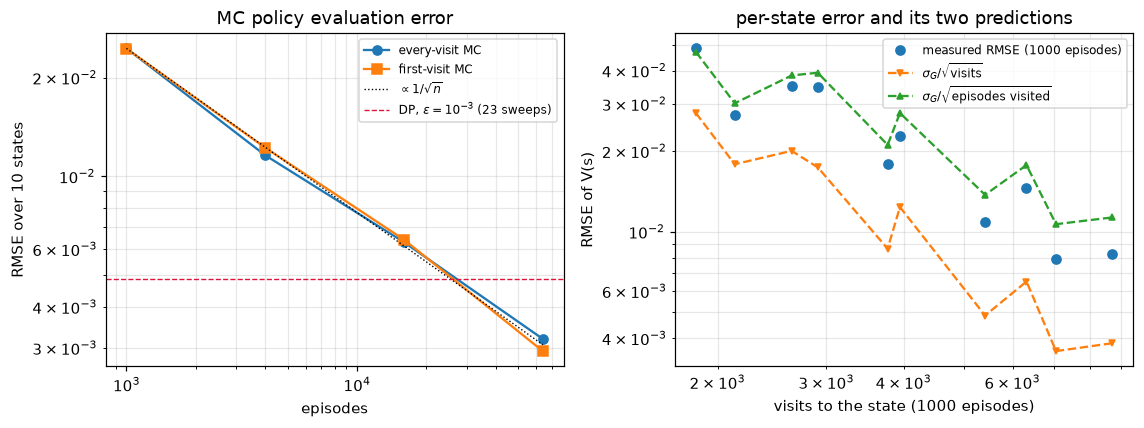
\includegraphics[width=\linewidth]{fig_mc_error.png}
\caption{왼쪽: 에피소드 수에 따른 MC 정책 평가의 RMSE(로그-로그). 점선이 $1/\sqrt{n}$ 기준선이고
가로 파선이 앞 장의 DP가 문턱 $10^{-3}$, $23$스윕에서 남긴 오차다. 두 곡선이 그 선을 만나는 자리가
$10^{5}$ 부근이다. 오른쪽: 상태별 오차를 두 가지 예측과 견준 것. 아래쪽 삼각형이 방문 횟수 기준
예측으로 실측을 두 배 낙관하고, 위쪽 삼각형이 에피소드 수 기준 예측으로 실측과 겹친다.
\texttt{ch05/paper/fig\_mc.py}에서 생성.}
\label{fig:mc-error}
\end{figure}

\subsection{고정값 \texorpdfstring{$\alpha$}{alpha}가 남기는 잔차}
\label{app:alpha}

본문의 [보충] ``고정값 $\alpha$가 남기는 바닥''이 쓴 근거다. 제어를 잠시 밀어 두고 무작위 정책 평가를
두 방식으로 $100{,}000$ 에피소드씩 돌린다. 평가할 정책이 고정되어 있으므로 $\alpha$를 쓸 이유가
전혀 없는 상황이며, 그래서 차이가 순수하게 드러난다.

\begin{table}[htbp]
\centering
\caption{$1/n$ 평균과 고정값 $\alpha$의 잔차($3\times4$ 그리드, 무작위 정책, $100{,}000$ 에피소드,
시드 $20$개). ``측정 표준편차''는 시드마다 얻은 $V(s)$의 시드 간 표준편차를 $10$개 상태에 대해
평균한 것이다. ``이론''은 $\alpha$ 행에서는 아래에서 유도하는 $\sqrt{\alpha/(2-\alpha)}\,\sigma_G$이고,
$1/n$ 행에서는 부록 \ref*{app:error-rate}의 $\sigma_G/\sqrt{m}$이다.}
\label{tab:alpha}
\small
\begin{tabular}{@{}lllll@{}}
\toprule
갱신 방식 & 측정 표준편차 & 이론 & 측정/이론 & RMSE \\
\midrule
$1/n$ 평균        & $0.00206$ & $0.00246$ & $0.84$ & $0.00241$ \\
$\alpha = 0.1$    & $0.23748$ & $0.15598$ & $1.52$ & $0.24097$ \\
$\alpha = 0.05$   & $0.16767$ & $0.10887$ & $1.54$ & $0.17164$ \\
$\alpha = 0.01$   & $0.07616$ & $0.04820$ & $1.58$ & $0.07836$ \\
\bottomrule
\end{tabular}
\end{table}

\paragraph{정상 상태의 분산.}
갱신식 $Q \leftarrow Q + \alpha(G-Q)$를 $Q \leftarrow (1-\alpha)Q + \alpha G$로 고쳐 쓰고 $G$들이
서로 독립이며 분산이 $\sigma_G^2$라 두면, 정상 상태에서의 분산은
\begin{equation*}
  \mathrm{Var}[Q_\infty] = \frac{\alpha}{2-\alpha}\,\sigma_G^2
\end{equation*}
이다. 이 값은 $n$과 무관하며, 여기서 폭 $\sqrt{\alpha/(2-\alpha)}\,\sigma_G$의 띠와 유효 표본 수
$n_{\text{eff}} = (2-\alpha)/\alpha$가 나온다.

표~\ref{tab:alpha}의 측정/이론이 $\alpha$ 세 값에서 $1.52$, $1.54$, $1.58$로 거의 같다는 것이 이
설명을 뒷받침한다. 상수배만큼 어긋나는 것은 부록~\ref{app:first-every}에서 본 그대로다. 위 식은
$G$들이 독립이라 가정했는데 한 에피소드 안의 방문들은 꼬리를 공유해 상관되어 있으므로 실제 분산이
그만큼 부풀려진다. 어긋남이 상수배에 그친다는 것은 $\alpha$에 대한 의존
$\sqrt{\alpha/(2-\alpha)}$가 그대로 맞는다는 뜻이며, 실제로 $\alpha$를 $0.1\to0.05$로 반으로 줄이면
측정 표준편차가 $0.2375 \to 0.1677$로 $1.416$배 줄어 $\sqrt{2}=1.414$와 맞는다.

\begin{figure}[htbp]
\centering
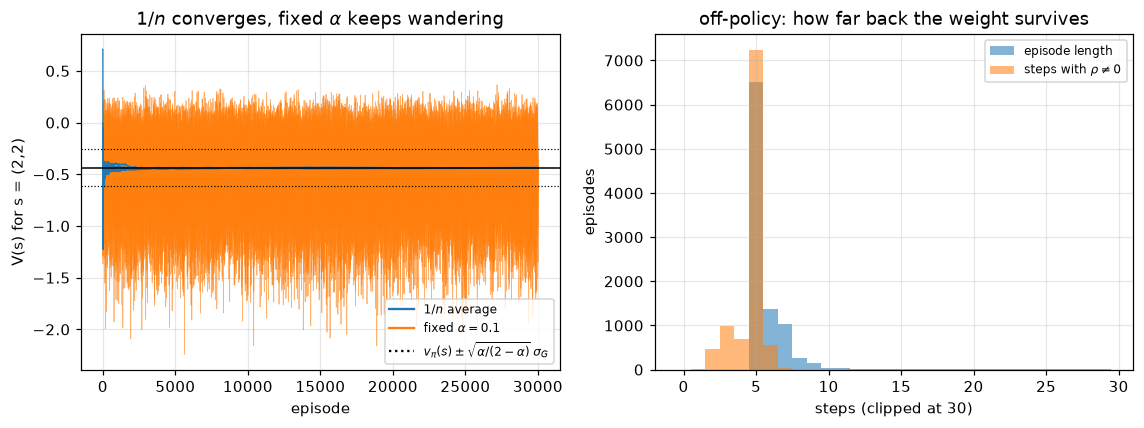
\includegraphics[width=\linewidth]{fig_mc_alpha_rho.png}
\caption{왼쪽: 상태 $(2,2)$의 추정치가 에피소드에 따라 움직이는 모습을 시드 여섯 개씩 겹쳐 그린 것.
파란 선($1/n$)은 참값(가로 실선)으로 모여 붙고 주황 선($\alpha=0.1$)은 점선으로 표시한
$\pm\sqrt{\alpha/(2-\alpha)}\,\sigma_G$의 띠 안에서 끝까지 서성인다. 오른쪽: 오프-정책 예제에서
에피소드 길이와 중요도 가중치가 살아 있는 꼬리 길이의 분포. 부록 \ref*{app:rho}에서 다룬다. \texttt{ch05/paper/fig\_mc.py}에서 생성.}
\label{fig:alpha-rho}
\end{figure}

\subsection{\texorpdfstring{$\varepsilon$}{eps}-탐욕 치우침의 몫 가르기}
\label{app:bias}

본문에서 온-정책 MC 제어의 $\max_a Q(s,a)$가 $v_*(s)$보다 작은 까닭을 $\varepsilon$ 몫과 표본 몫으로
나누어 적었다. 그 가름의 근거다.

\begin{table}[htbp]
\centering
\caption{치우침을 두 몫으로 가르기. 실측은 모두 시드 $20$개의 평균이다. 학습을 $40$배로 늘리면
$-0.05$ 근처에서 더 내려가지 않고, 초깃값을 $v_*$ 위쪽인 $1.0$으로 올리면 크기가 줄면서 부호도
흩어진다. 초깃값과 방문 부족이 실재하는 몫이라는 뜻이다.}
\label{tab:bias-split}
\small
\begin{tabular}{@{}lrr@{}}
\toprule
 & 평균 차이 & 음수인 시드 \\
\midrule
$\varepsilon=0.1$ 목표의 이론값(표본 없음) & $-0.0235$ & --- \\
\midrule
$10{,}000$ 에피소드, $Q$ 초깃값 $0$   & $-0.1021$ & $100\%$ \\
$100{,}000$ 에피소드                  & $-0.0525$ & $100\%$ \\
$400{,}000$ 에피소드                  & $-0.0513$ & $100\%$ \\
$10{,}000$ 에피소드, $Q$ 초깃값 $1.0$ & $-0.0651$ & $80\%$ \\
\bottomrule
\end{tabular}
\end{table}

내려가다 멈추는 자리가 이론값 $-0.0235$가 아니라 $-0.05$ 근처인 까닭은 방문이 고르지 않아서다.
$10{,}000$ 에피소드에서 시작 상태 $(2,0)$은 $13{,}314$번 지나는데 폭탄 칸 $(1,3)$은 $54$번뿐이라
$250$배가 벌어지고, 칸별 치우침도 $(0,2)$의 $-0.0000$부터 $(2,3)$의 $-0.3193$까지 방문 횟수를
따라간다. 목표에서 먼 칸 몇 개가 평균을 끌어내리고 있는 것이다.

\subsection{중요도 가중치 \texorpdfstring{$\rho$}{rho}가 취하는 값}
\label{app:rho}

본문의 [보충] ``$\rho$는 0 아니면 폭발''이 쓴 근거다. 대상 정책 $\pi$는 한 행동에 $1$, 나머지 셋에
$0$을 준다. 행동 정책은 $\varepsilon=0.1$이므로 탐욕 행동에 $\varepsilon/4 + (1-\varepsilon) =
0.925$, 나머지에 $\varepsilon/4 = 0.025$를 준다. 한 걸음의 가중치 $\pi(a\mid s)/b(a\mid s)$가 가질
수 있는 값이 그 조합으로 정해진다.
\begin{equation*}
  \frac{\pi(a\mid s)}{b(a\mid s)} =
  \begin{cases}
    0                        & a \neq \text{$\pi$의 탐욕 행동} \quad (\text{네 번 중 세 번}),\\[2pt]
    1/0.925 = 1.081          & a = \text{$\pi$와 $b$의 탐욕 행동이 같을 때},\\[2pt]
    1/0.025 = 40             & a = \text{$\pi$의 탐욕 행동이지만 $b$의 것과 다를 때}.
  \end{cases}
\end{equation*}

세 번째 줄이 생기는 자리가 동점 처리다. \lstinline|update()|는 \lstinline|greedy_probs()|를 $\pi$용과
$b$용으로 두 번 부르는데, 함수 안의 \lstinline|argmax()|는 동점이면 무작위로 하나를 고른다. 두 번의
호출이 서로 다른 행동을 뽑으면 $\pi$가 $1$을 준 행동에 $b$는 $0.025$만 주고, 가중치가 단숨에 $40$배로
뛴다. $Q$가 모두 $0$인 학습 초기에 네 행동이 전부 동점이므로 그 시기에 몰려서 나타난다.

\begin{table}[htbp]
\centering
\caption{한 걸음 가중치가 실제로 취한 값(시드 $0$, $10{,}000$ 에피소드, 갱신 $134{,}820$회).
$1.0$은 아직 한 번도 갱신되지 않아 $\pi$와 $b$가 모두 초기 균등분포로 남아 있는 첫 에피소드의
걸음들이다. $40$배가 몇 번 나오는지는 동점이 언제 풀리느냐에 달려 시드마다 크게 다르며, 시드
$10$개에서 $11$회부터 $3{,}972$회까지 나타났다.}
\label{tab:rho-values}
\small
\begin{tabular}{@{}lrrl@{}}
\toprule
가중치 & 횟수 & 비율 & 언제 \\
\midrule
$0$      & $80{,}045$ & $59.37\%$ & 걸은 행동이 $\pi$의 탐욕 행동이 아닐 때 \\
$1.081$  & $54{,}740$ & $40.60\%$ & 두 정책의 탐욕 행동이 같을 때 \\
$40$     & $25$       & $0.02\%$  & 동점을 두 호출이 다르게 풀었을 때 \\
$1.0$    & $10$       & $0.01\%$  & 첫 에피소드, 두 정책이 아직 균등분포일 때 \\
\bottomrule
\end{tabular}
\end{table}

가중치가 살아 있는 구간이 얼마나 짧은지는 그림~\ref{fig:alpha-rho} 오른쪽에 있다. 에피소드 길이는
평균 $9.9$$\sim$$13.5$걸음에 중앙값 $5$걸음이고 시드에 따라 $20{,}000$걸음이 넘는 것도 나오는데,
$\rho \neq 0$인 꼬리는 평균 $4.65$걸음이고 시드 $10$개를 통틀어 $8$걸음을 넘은 적이 없다. 누적
$\rho$의 최댓값도 시드에 따라 $1.6$에서 $63.9$까지 튀었다.


% =============================================================================
\section*{재현 정보}
\addcontentsline{toc}{section}{재현 정보}
% =============================================================================

본고의 수치는 세 갈래에서 나왔다.

\emph{정확한 값}(표~\ref{tab:eps-gap}, 표~\ref{tab:is-var}, 그리고 $v_*$와 $v_\pi$)은 표본을 쓰지
않고 계산한 것이다. 그리드 월드의 가치 함수는 앞 장의 반복적 정책 평가와 가치 반복법을 갱신 폭이
$10^{-14}$ 아래로 떨어질 때까지 돌려 얻었고, 중요도 샘플링의 분산은 값이 셋뿐이라 직접 더했다.

\emph{예제 코드의 실측}(표~\ref{tab:control}, 표~\ref{tab:alpha-control},
표~\ref{tab:bias-split}, 표~\ref{tab:on-vs-off}, 표~\ref{tab:rho-values},
표~\ref{tab:three})은 \texttt{ch05/}의 예제를 그대로 돌리고 계측만 덧붙인 것이다. 온-정책은 \texttt{s03\_mc\_control.py}의 \lstinline|np.argmax| 판본을, 오프-정책은
\texttt{s05\_mc\_control\_offpolicy.py}가 부르는 \texttt{common/utils.py}의 무작위 동점 처리
판본을 쓴다. 두 파일의 동점 처리가 서로 다르다는 점은 $\varepsilon$-탐욕 정책 절에 적었고,
표~\ref{tab:rho-values}의 $40$배 가중치가 거기서 나온다. 시드는 \lstinline|np.random.seed()|에 $0$부터 차례로 넣었고, 항목 대부분이 $50$개다.
학습 길이를 $40$배까지 늘리는 표~\ref{tab:bias-split}은 계산 시간 때문에 $20$개,
$\rho$ 통계인 표~\ref{tab:rho-values}는 계측 비용 때문에 $10$개다.
표~\ref{tab:is-measured}는 예제 코드의 뽑기를 $n=100$씩 $10{,}000$번 되풀이한 것이다.

\emph{그림의 실측}(그림~\ref{fig:mc-error}, 그림~\ref{fig:alpha-rho})은
\texttt{ch05/paper/fig\_mc.py}로 생성한다. 에피소드를 수십만 번 돌려야 해서 환경의 전이를 미리 표로
펼치고 역누적분포로 표본을 뽑는 빠른 판본을 쓰지만, 갱신식과 정책은 예제와 같다.

시드를 바꾸면 값이 달라지는 항목과 그렇지 않은 항목을 섞지 않았다. 표에 ``평균''이라 적힌 것은
시드에 따라 흔들리는 값이고, 흔들리는 폭이 논의에 중요한 자리에서는 범위를 함께 적었다.

\begin{thebibliography}{9}
\bibitem{dlfs4}
사이토 고키, \emph{밑바닥부터 시작하는 딥러닝 4: 파이썬으로 구현하는 강화 학습 알고리즘}, 한빛미디어, 2023.
\bibitem{ch04}
sajacaros, \emph{동적 프로그래밍: 벨만 방정식의 등호를 갱신식으로 바꿔 읽기}, 2026.
\bibitem{sutton}
R.~S. Sutton and A.~G. Barto, \emph{Reinforcement Learning: An Introduction}, 2nd ed., MIT Press, 2018.
\bibitem{ulam}
S.~M. Ulam, \emph{Adventures of a Mathematician}, Charles Scribner's Sons, 1976.
\bibitem{metropolis}
N.~Metropolis, ``The Beginning of the Monte Carlo Method,'' \emph{Los Alamos Science}, Special Issue, pp.~125--130, 1987.
\bibitem{singh}
S.~P. Singh and R.~S. Sutton, ``Reinforcement Learning with Replacing Eligibility Traces,''
\emph{Machine Learning}, vol.~22, pp.~123--158, 1996.
\end{thebibliography}

\vspace{4mm}
\noindent\rule{\linewidth}{0.4pt}\\
\footnotesize
본 문서에 실린 그림 중 ``원서 그림''으로 표기한 것은 참고문헌~\cite{dlfs4}의 도판이며, 학습 정리 목적으로
인용하였다. 그 밖의 그림과 표는 본고에서 직접 생성한 것이다.

\end{document}
